\documentclass[oneside, a4paper, onecolumn, 11pt]{article}

\usepackage[usenames,dvipsnames,svgnames,table]{xcolor}
\usepackage{sectsty}
\chapterfont{\color{blue}}  % sets colour of chapters
\sectionfont{\color{cyan}}  % Cerulean
\subsectionfont{\color{ProcessBlue}}  % MidnightBlue, CornflowerBlue, NavyBlue ProcessBlue

\usepackage{amsmath, amssymb}
\usepackage{booktabs, bm}           %%  bold math
\usepackage{cancel}
\usepackage{dcolumn}  %%  Align table columns on decimal point
\usepackage{epsfig, epsf, eurosym, enumitem}
\usepackage{fancyhdr}
\usepackage[T1]{fontenc}
\usepackage[para]{footmisc}
\usepackage{graphicx }
%\usepackage{lscape}
\usepackage{hyperref,ifthen}
\usepackage{mathptmx, multicol}
\usepackage[authoryear, round]{natbib}
\usepackage{nopageno}
\usepackage{subfigure}
\usepackage{verbatim}
\usepackage{threeparttable}
\usepackage[usenames,dvipsnames]{xcolor}
\usepackage{tcolorbox}
\usepackage{tabularx}
\usepackage{array}
\usepackage{colortbl}
\usepackage{framed}
\usepackage{todonotes}



%%%%%%%%%%%%%%%%%%%%%%%%%%%%%%%%%%%%%%%%%%%
%       define Journal abbreviations      %
%%%%%%%%%%%%%%%%%%%%%%%%%%%%%%%%%%%%%%%%%%%
\def\nat{Nat} \def\apjl{ApJ~Lett.} \def\apj{ApJ}
\def\apjs{ApJS} \def\aj{AJ} \def\mnras{MNRAS}
\def\prd{Phys.~Rev.~D} \def\prl{Phys.~Rev.~Lett.}
\def\plb{Phys.~Lett.~B} \def\jhep{JHEP}
\def\npbps{NUC.~Phys.~B~Proc.~Suppl.} \def\prep{Phys.~Rep.}
\def\pasp{PASP} \def\aap{Astron.~\&~Astrophys.} \def\araa{ARA\&A}
\def\jcap{\ref@jnl{J. Cosmology Astropart. Phys.}} 
\def\nar{New~A.R.} \def\aapr{A\&ARv}

\newcommand{\preep}[1]{{\tt #1} }

%%%%%%%%%%%%%%%%%%%%%%%%%%%%%%%%%%%%%%%%%%%%%%%%%%%%%
%              define symbols                       %
%%%%%%%%%%%%%%%%%%%%%%%%%%%%%%%%%%%%%%%%%%%%%%%%%%%%%
\def \Mpc {~{\rm Mpc} }
\def \Om {\Omega_0}
\def \Omb {\Omega_{\rm b}}
\def \Omcdm {\Omega_{\rm CDM}}
\def \Omlam {\Omega_{\Lambda}}
\def \Omm {\Omega_{\rm m}}
\def \ho {H_0}
\def \qo {q_0}
\def \lo {\lambda_0}
\def \kms {{\rm ~km~s}^{-1}}
\def \kmsmpc {{\rm ~km~s}^{-1}~{\rm Mpc}^{-1}}
\def \hmpc{~\;h^{-1}~{\rm Mpc}} 
\def \hkpc{\;h^{-1}{\rm kpc}} 
\def \hmpcb{h^{-1}{\rm Mpc}}
\def \dif {{\rm d}}
\def \mlim {m_{\rm l}}
\def \bj {b_{\rm J}}
\def \mb {M_{\rm b_{\rm J}}}
\def \mg {M_{\rm g}}
\def \mi {M_{\rm i}}
\def \qso {_{\rm QSO}}
\def \lrg {_{\rm LRG}}
\def \gal {_{\rm gal}}
\def \xibar {\bar{\xi}}
\def \xis{\xi(s)}
\def \xisp{\xi(\sigma, \pi)}
\def \Xisig{\Xi(\sigma)}
\def \xir{\xi(r)}
\def \max {_{\rm max}}
\def \gsim { \lower .75ex \hbox{$\sim$} \llap{\raise .27ex \hbox{$>$}} }
\def \lsim { \lower .75ex \hbox{$\sim$} \llap{\raise .27ex \hbox{$<$}} }
\def \deg {^{\circ}}
%\def \sqdeg {\rm deg^{-2}}
\def \deltac {\delta_{\rm c}}
\def \mmin {M_{\rm min}}
\def \mbh  {M_{\rm BH}}
\def \mdh  {M_{\rm DH}}
\def \msun {M_{\odot}}
\def \z {_{\rm z}}
\def \edd {_{\rm Edd}}
\def \lin {_{\rm lin}}
\def \nonlin {_{\rm non-lin}}
\def \wrms {\langle w_{\rm z}^2\rangle^{1/2}}
\def \dc {\delta_{\rm c}}
\def \wp {w_{p}(\sigma)}
\def \PwrSp {\mathcal{P}(k)}
\def \DelSq {$\Delta^{2}(k)$}
\def \WMAP {{\it WMAP \,}}
\def \cobe {{\it COBE }}
\def \COBE {{\it COBE \;}}
\def \HST  {{\it HST \,\,}}
\def \Spitzer  {{\it Spitzer \,}}
\def \ATLAS {VST-AA$\Omega$ {\it ATLAS} }
\def \BEST   {{\tt best} }
\def \TARGET {{\tt target} }
\def \TQSO   {{\tt TARGET\_QSO}}
\def \HIZ    {{\tt TARGET\_HIZ}}
\def \FIRST  {{\tt TARGET\_FIRST}}
\def \zc {z_{\rm c}}
\def \zcz {z_{\rm c,0}}


\newcommand{\sqdeg}{deg$^{-2}$}
\newcommand{\lya}{Ly$\alpha$\ }
%\newcommand{\lya}{Ly\,$\alpha$\ }
\newcommand{\lyaf}{Ly\,$\alpha$\ forest}
%\newcommand{\eg}{e.g.~}
%\newcommand{\etal}{et~al.~}
\newcommand{\cii}{C\,{\sc ii}\ }
\newcommand{\ciii}{C\,{\sc iii}]\ }
\newcommand{\civ}{C\,{\sc iv}\ }
\newcommand{\SiIV}{Si\,{\sc iv}\ }
\newcommand{\mgii}{Mg\,{\sc ii}\ }
\newcommand{\feii}{Fe\,{\sc ii}\ }
\newcommand{\feiii}{Fe\,{\sc iii}\ }
\newcommand{\caii}{Ca\,{\sc ii}\ }
\newcommand{\halpha}{H\,$\alpha$\ }
\newcommand{\hbeta}{H\,$\beta$\ }
\newcommand{\oi}{[O\,{\sc i}]\ }
\newcommand{\oii}{[O\,{\sc ii}]\ }
\newcommand{\oiii}{[O\,{\sc iii}]\ }
\newcommand{\heii}{[He\,{\sc ii}]\ }
\newcommand{\nii}{N\,{\sc ii}\ }
\newcommand{\nv}{N\,{\sc v}\ }

%% From:: /cos_pc19a_npr/LaTeX/proposals/JWST/JWST_ERS/Proposal/lines.tex
%%  
\newcommand{\imw}{$i$--$W3$}
\newcommand{\imwf}{$i$--$W4$}
\newcommand{\rmwf}{$r$--$W4$}
\newcommand{\imwt}{$i$--$W2$}
\newcommand{\wtmwf}{$W3$--$W4$}
%\newcommand{\kms}{km s$^{-1}$}
\newcommand{\cmN}{cm$^{-2}$}
\newcommand{\cmn}{cm$^{-3}$}
%\newcommand{\msun}{M$_{\odot}$}
\newcommand{\lsun}{L$_{\odot}$}
\newcommand{\lam}{$\lambda$}
\newcommand{\mum}{$\mu$m}
\newcommand{\ebv}{$E(B$$-$$V)$}
%\newcommand{\heii}{\mbox{He\,{\sc ii}}}
\newcommand{\cv}{\mbox{C\,{\sc v}}}
%\newcommand{\civ}{\mbox{C\,{\sc iv}}}
%\newcommand{\ciii}{\mbox{C\,{\sc iii}}}
%\newcommand{\cii}{\mbox{C\,{\sc ii}}}
%\newcommand{\nv}{\mbox{N\,{\sc v}}}
\newcommand{\niv}{\mbox{N\,{\sc iv}}}
\newcommand{\niii}{\mbox{N\,{\sc iii}}}
%\newcommand{\oi}{\mbox{O\,{\sc i}}}
%\newcommand{\oii}{\mbox{O\,{\sc ii}}}
%\newcommand{\oiii}{\mbox{[O\,{\sc iii}]}}
\newcommand{\oiv}{\mbox{O\,{\sc iv}}}
\newcommand{\ov}{\mbox{O\,{\sc v}}}
\newcommand{\ovi}{\mbox{O\,{\sc vi}}}
\newcommand{\ovii}{\mbox{O\,{\sc vii}}}

%\newcommand{\feii}{\mbox{Fe\,{\sc ii}}}
%\newcommand{\feiii}{\mbox{Fe\,{\sc iii}}}
%\newcommand{\mgii}{\mbox{Mg\,{\sc ii}}}
\newcommand{\neii}{[Ne\,{\sc ii}]\ }
\newcommand{\neiii}{[Ne\,{\sc ii}]\ }
\newcommand{\nev}{Ne\,{\sc v}\ }
\newcommand{\nevi}{[Ne\,{\sc vi}]\ }
\newcommand{\neviii}{\mbox{Ne\,{\sc viii}}}
\newcommand{\aliii}{\mbox{Al\,{\sc iii}}}
\newcommand{\siii}{\mbox{Si\,{\sc ii}}}
\newcommand{\siiii}{\mbox{Si\,{\sc iii}}}
\newcommand{\siiv}{\mbox{Si\,{\sc iv}}}
%\newcommand{\lya}{\mbox{Ly$\alpha$}}
%\newcommand{\lyb}{\mbox{Ly$\beta$}}
\newcommand{\hi}{\mbox{H\,{\sc i}}}
\newcommand{\snine}{\mbox{[S\,{\sc ix}]}}
\newcommand{\sivi}{\mbox{[Si\,{\sc vi}]}}
\newcommand{\sivii}{\mbox[{Si\,{\sc vii}]}}
\newcommand{\siix}{\mbox{[Si\,{\sc ix}]}}
\newcommand{\six}{\mbox{[Si\,{\sc x}]}}
\newcommand{\sixi}{\mbox{[Si\,{\sc xi}]}}
\newcommand{\caviii}{\mbox{[Ca\,{\sc viii}]}}
\newcommand{\arii}{\mbox{[Ar\,{\sc ii}]}}

%%[Ar II] 6.97
%% [S IX] 1.252 μm 328 
% [Si X] 1.430 μm 351 
% [Si XI] 1.932 μm 401 
% [Si VI] 1.962 μm 167 
% [Ca VIII] 2.321 μm 128 
% [Si VII] 2.483 μm 205 
% [Si IX] 3.935 μm 303
% [Ar II] 6.97


%\snine\ at 1.252$\mu$m, \six\ at 1.430$\mu$m, \sixi\ at 1.932$\mu$m, \sivi\ at
%1.962$\mu$m, \caviii\ at 2.321$\mu$m, \sivi\ at 2.483$\mu$m \siix\ at
%3.935$\mu$m and \arii\ at 6.97$\mu$m. 
%%
%% such as [Ne ii]12.8 μm, [Ne v]14.3 μm, [Ne iii]15.5 μm, [S iii]18.7 μm and 33.48 μm, [O iv]25.89 μm and [Si ii]34.8 μm (e.g
%%
%% MIR emission lines like [NeII] and [NeV] are ..
%%
%% Also,  arXiv:astro-ph/0003457v1 
%% [NeV] 14.32um & 24.32um and [NeVI] 7.65um imply an A(V)>160 towards the NLR...
%% [NeIII]15.56um/[NeII]12.81um
%%
%% [Ne V] 14.3, 24.2 μm 97.
%% [Ne II] 12.8 μm
%% [OIV] 26μm
%%


%\usepackage[left=2.05cm,top=2.05cm,bottom=1.55cm,right=2.05cm]{geometry}
\usepackage[left=2.05cm,top=2.05cm,right=2.05cm]{geometry}
\setlength{\bibsep}{0.0pt}


\tcbuselibrary{skins}
\newcolumntype{Y}{>{\raggedleft\arraybackslash}X}

\tcbset{tab1/.style={enhanced, fonttitle=\bfseries, fontupper=\normalsize\sffamily,
colback=yellow!10!white,
colframe=red!50!black,
colbacktitle=Cerulean!40!white,
coltitle=black,center title}
%subtitle style={boxrule=0.4pt, colback=yellow!50!red!25!white} 
}

%% To fix list things: 
\setitemize{noitemsep,topsep=0pt,parsep=0pt,partopsep=0pt,leftmargin=*}
\renewcommand{\labelitemi}{\tiny$\blacksquare$}

\renewcommand{\thesection}{\alph{section}}
%\renewcommand{\thesubsection}{\Alph{subsection}}

\pagestyle{fancy}
%\renewcommand{\headrulewidth}{0pt}  %% Remove line at top

%\pagestyle{empty}
\fancyhf{}
%\lhead{{\it ERC-2015-StG}}
%\lhead{{\it DEQUASARS: Part B1 }}
\lhead{{\it Ross}}
\chead{Part B2}
\rhead{Q4D}
\setcounter{page}{1}
\lfoot{{\it ERC-COG-2018}}
\rfoot{{\it Scientific Proposal}}
\cfoot{{\it Page \thepage\ of 15}}
%\rfoot{{\it FP7-PEOPLE-2013-IIF}}

\newenvironment{itemize*}%
  {\begin{itemize}%
    \setlength{\itemsep}{0pt}%
    \setlength{\parskip}{0pt}}%
  {\end{itemize}}


\begin{document}

\begin{center}
{\Large \bf \textcolor{Cerulean}{Q4D: Quasars in the 4th Dimension\\}}
%\vspace{4pt} 
 %{\Large \bf \textcolor{Cerulean}{the new field of Extragalactic Variable Astrophysics} }
\end{center}
\vspace{-16pt} 


%\tableofcontents


%\medskip \medskip 
\medskip \medskip
%\begin{quotation}
\noindent
{\it 
All massive galaxies are thought to have supermassive black holes at
their centres, and to have undergone a ``quasar phase'' in
their past. Along with fusion in stars, accretion onto the central
supermassive black hole is the main energy source available to a
galaxy. However, we are missing a deep understanding of galaxy
formation theory since we still do not understand in key detail how
the energy associated with the quasar escapes the central engine to impact the host galaxy and
the intergalactic medium. Further issues arise since recent
observations of extreme variability in quasars have broken standard
viscous accretion disk models.

\smallskip
\smallskip
\noindent
In this proposal, we propose the ground breaking idea of combining the
data from several next-generation state-of-the art surveys (SDSS-V,
DESI, LSST, 4MOST, ESA {\it Euclid} and JWST) in order to go beyond
the state-of-the-art and construct the extragalactic dataset with the
crucial time-domain aspect that is necessary to address the current
challenges.  The experience of the P.I., along with the strategic
data nexus aspect of the Royal Observatory at the University of
Edinburgh makes my group uniquely placed to address and answer this
problem.  The goal is to create a holistic theory of accretion disk
physics and quasar feedback in galaxy formation theory. We are also
extremely well placed to discover brand new extragalactic variable
phenomena.
}
%\end{quotation}
\vspace{-20pt}


\section{State-of-the-art and Objectives}
\vspace{-4pt}

\subsection{Background}
\noindent
Quasars\footnote{ Historically, ``quasars'' and ``Active Galactic
Nuclei (AGN)'' have described different luminosity/classes of objects,
but here we use these terms interchangeably (with a preference for
quasar) in recognition of the fact that they both describe accreting
supermassive black holes \citep[e.g.][]{Haardt2016book}.}  are powered
by accretion of material onto supermassive black holes (SMBHs), via
accretion disks.  In the local Universe, there is a link between the
key properties of massive galaxies, such as bulge mass, and their
central supermassive black holes \citep[e.g., ][]{McLure_Dunlop2002,
HaringRix2004, Salviander2007, Greene2010, KormendyHo2013}. This has
led to the hypothesis that the supermassive black hole, when accreting,
has an influence on its host galaxy by the means of some regulatory
``feedback'' mechanism(s) \citep[e.g., ][]{Sijacki2007, Hopkins2008a,
AlexanderHickox2012, Fabian2012, KingPounds2015}. However, the details
of the physical processes involved in this `AGN/quasar feedback' are
still disputed and, moreover, direct observational evidence for quasar
feedback in the early universe is conspicuous by its absence
\citep[e.g., ][]{HeckmanBest2014, NaabOstriker2017}. Hence, a major
source of uncertainty in our current understanding of galaxy evolution
is how supermassive black holes influence, and potentially regulate,
their host galaxies \citep{Vogelsberger2013, Vogelsberger2014,
Schaye2015, Angles-Alcazar2013, Angles-Alcazar2017}.


\smallskip 
\smallskip
\noindent
Furthermore, the details of the physical processes involved in the
quasar activity including how the SMBH directly couples and affects
its most local environment, i.e., the accretion disk, broad line
region and dusty torus, are still unknown at this point
\citep[e.g.,][]{Netzer2015, Padovani2017}.

\smallskip 
\smallskip
\noindent
Although it has long been established that quasars are powered by
accretion discs surrounding supermassive black holes, there have also
been long-standing issues. For example, the observed spectral energy
distributions (SEDs) of typical quasars
\citep[e.g.,][]{Koratkar_Blaes1999, Sirko_Goodman2003} differ markedly
from classical predictions \citep[][]{SS73, Pringle1981} with a
typical observed quasar SED flat in $\lambda F_{\lambda}$ over several
decades in wavelength \citep{Elvis1994, Richards2006b}.  Also, real
accretion disks seem to be cooler \cite[e.g., ][]{Lawrence2012} and
larger \cite[e.g.,][]{Pooley2007, Morgan2010, Morgan2012,
Mosquera2011} than the standard accretion disk model predictions.

\smallskip 
\smallskip
\noindent
However, even more troubling are new observations of {\it extreme
variability} in some objects (see next section) - factors of several
over a decade or so, including, crucially, at optical wavelengths, and
not just in the extreme UV or in X-rays. This has led to the ``Quasar
Viscosity Crisis'' \citep{Lawrence2018}.

\smallskip 
\smallskip
\noindent
{\bf As such, we are left in the uncomfortable current situation of
invoking galaxy-wide ``quasar feedback'' in order to reconcile
demographic observations in cosmological-scale simulations, but where
we currently do not understand the physics of mechanism that is
supposed to initiate this necessary and vital energy transport.}


\subsubsection{Observational State-of-the-Art}
Here I present a concise overview of the observational
state-of-the-art in the brand new field of variable extragalactic
astrophysics, concentrating on quasar studies.

\smallskip
\smallskip
\noindent
\textbf{\textsc{A microscope for rapid Central Engines:}}
``Changing-look'' quasars \citep[CLQs; ][]{LaMassa2015,
Runnoe2016, Ruan2016, Runco2016, MacLeod2016, Yang2017} 
are defined to be luminous quasars which have a
dramatic appearance, or disappearance, of their broad emission-line
component on observed-frame month-to-year timescales.  CLQs are
important since they offer a direct observational probe into the
physical processes dictating the structure of the broad-line region
(BLR). These timescales can potentially be associated with the viscous
timescale (the drift time through the accretion disk), the light
crossing timescale (critical for reverberation mapping and disk
reprocessing) and the dynamical timescale of the BLR.  {\it CLQs are thus
an ideal laboratory for studying accretion physics, as the entire
system responds to a large change in ionizing flux on a human
timescale.}

\smallskip 
\smallskip
\noindent 
In \citet{MacLeod2016} I co-led the first systematic search for CLQs
based on photometry from SDSS and Pan-STARRS1, along with repeat
spectra from the SDSS/BOSS, and reported the discovery of 10
CLQs. This is a startling result since we now estimate
$\approx$10-15\% of bona fide quasars may exhibit `changing look'
behaviour on $\sim$10 year (rest-frame) timescales. However, plausible
time-scales for variable dust extinction are factors of $2-10$ too
long to explain the dimming and brightening in these sources.  Changes
in accretion rate are the currently favored explanation for CLQs, but
then the question of how the inner accretion disk couples to the BLR
immediately arises. Further investigation is thus warranted.

\begin{figure}[h]
  \begin{center}
    \hspace{-0.5cm}
    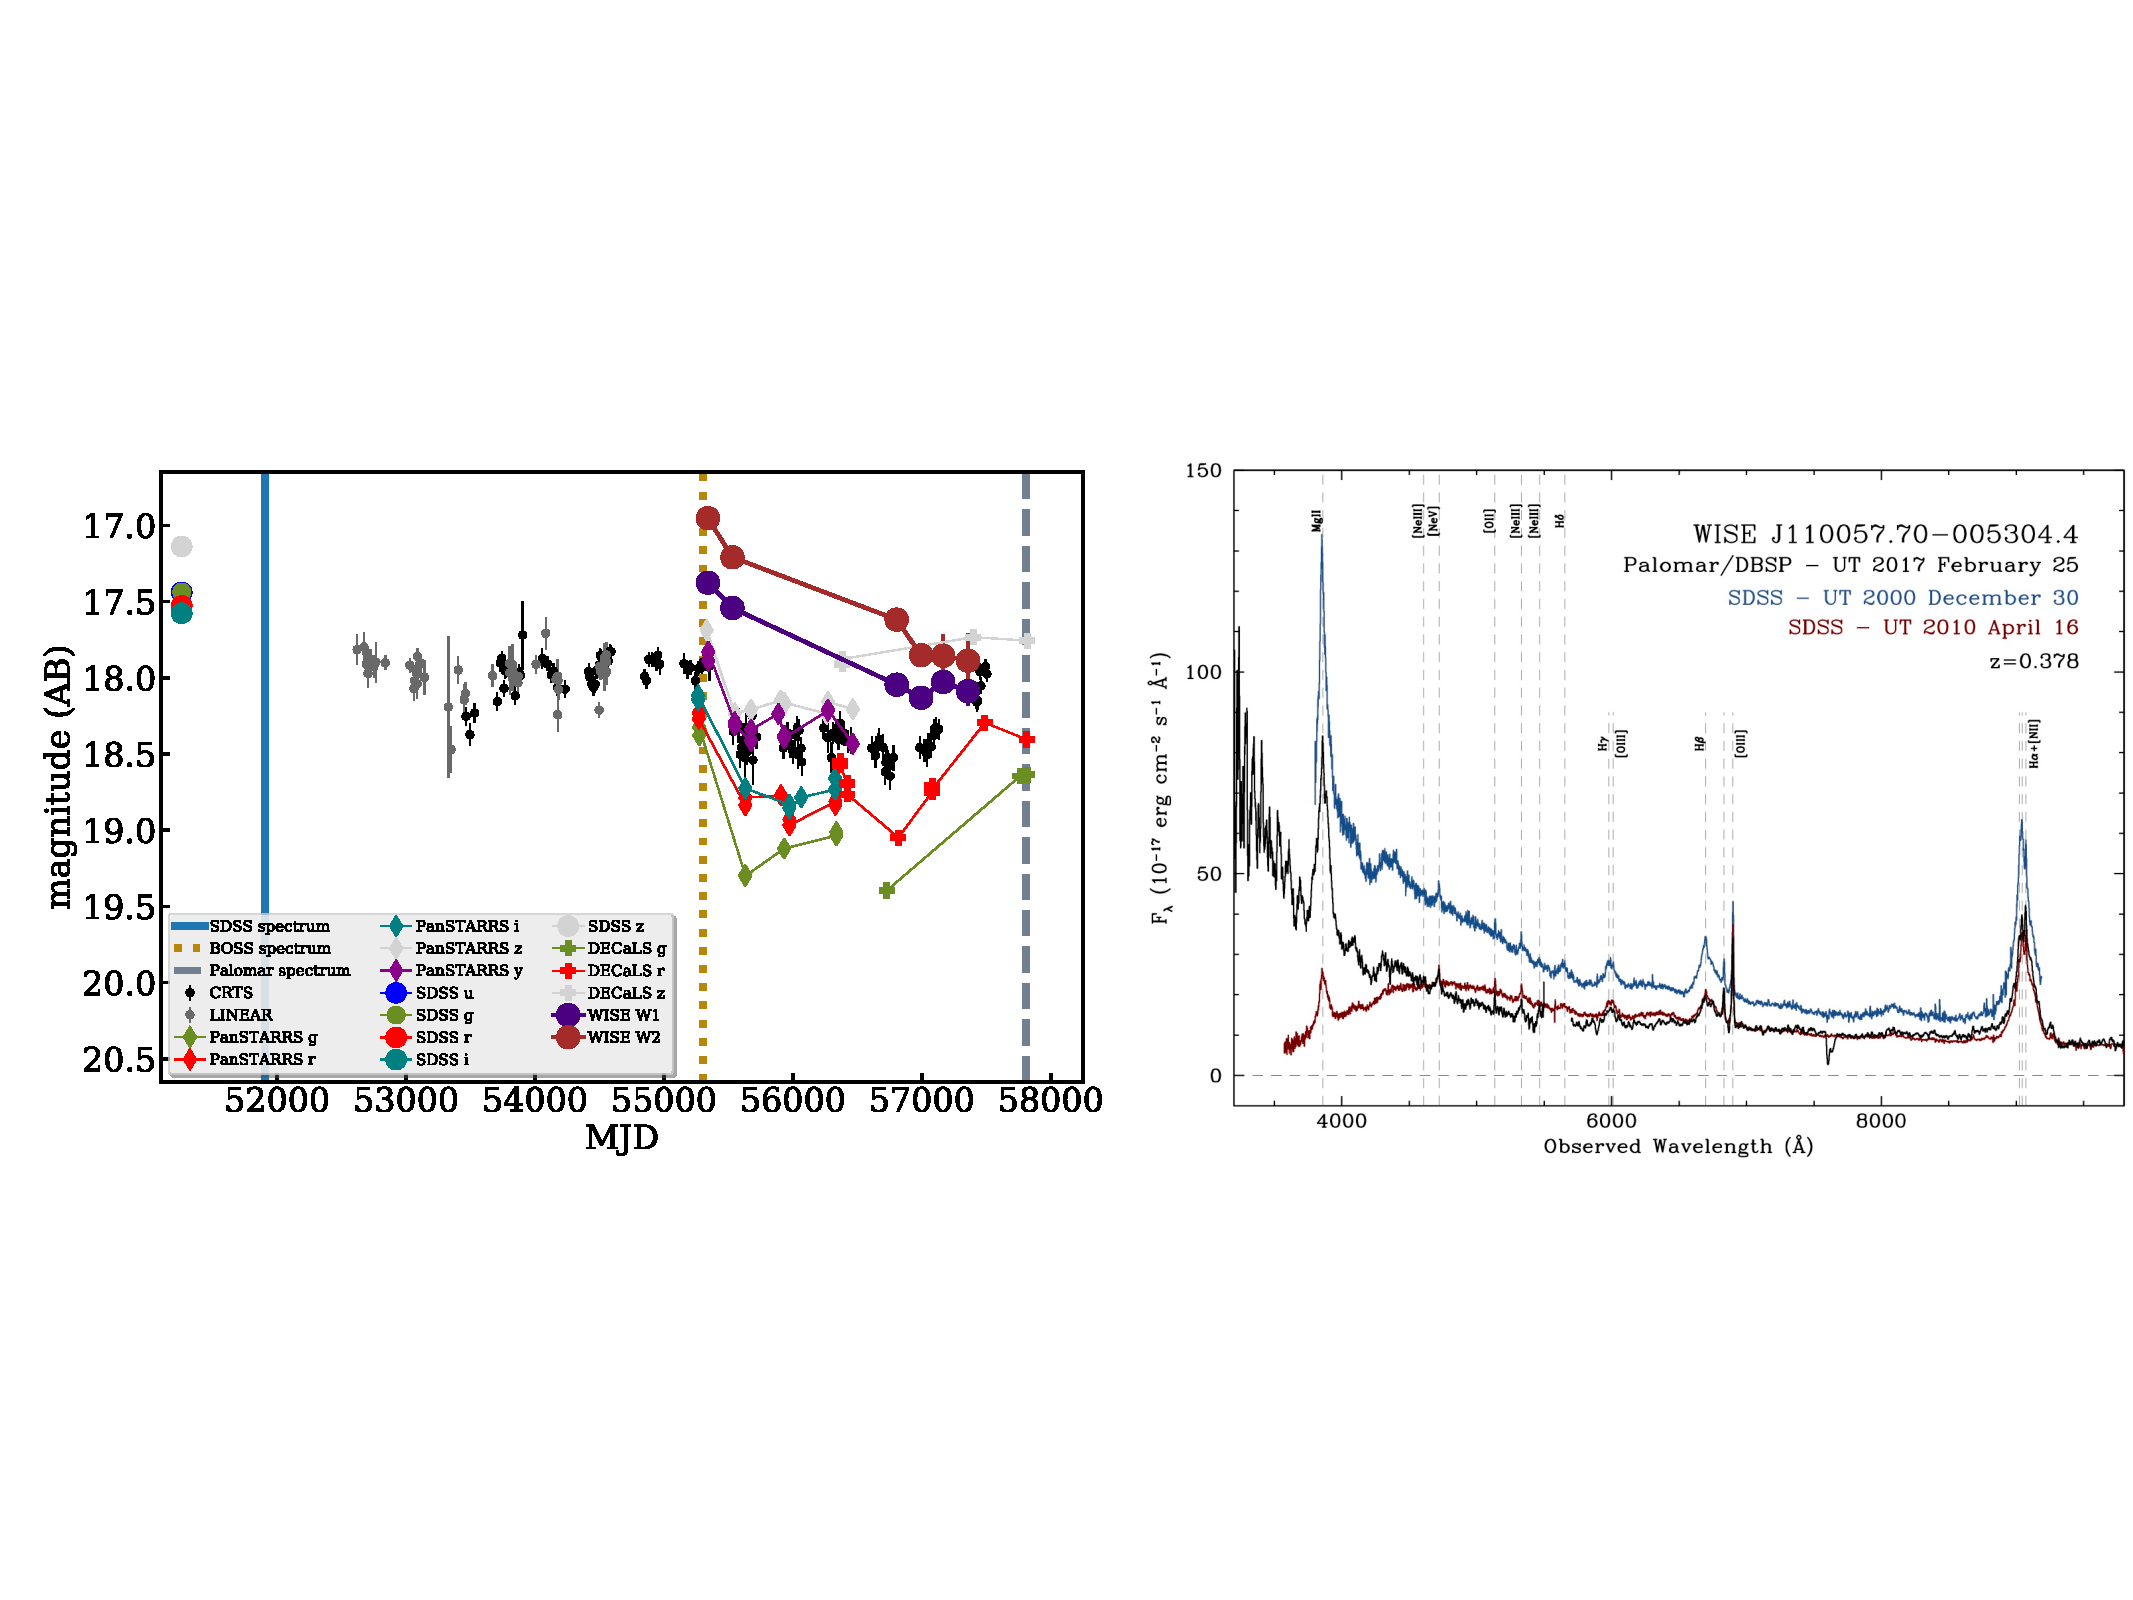
\includegraphics[height=6.25cm,width=17.2cm]
    {figures/J110057_LC_Spectra_20171024.pdf}
    \vspace{-10pt}
    \caption{\footnotesize 
      {\it (Left:)} The optical and infrared light-curve for
      J1100-0053; Note the fall in the infrared, whereas there is a
      decrease, but then recovery in the optical.  {\it (Right:)} Three
      epochs of spectra for J1100-0053.  The spectacular downturn in the
      blue for the 2010 spectrum indicates a dramatic change in the
      accretion disk.}
    \vspace{-16pt}
    \label{fig:J1100}
  \end{center}
\end{figure}

\smallskip
\smallskip
\noindent
\textbf{\textsc{New IR investigations into the CLQ Population:}}
Taking advantage of new optical imaging data from the Dark Energy
Camera Legacy Survey \href{http://legacysurvey.org/decamls/}{(DECaLS)}
and new IR light-curves from NEOWISE \citep{Meisner2017a,
Meisner2017b}, I have made further in-roads into understanding the CLQ
population. This includes identifying objects with rapidly changing IR
light-curves and also accretion disk changes, e.g. the $z=0.378$
quasar SDSS J110057-005304, see Figure~\ref{fig:J1100}. From
J1100-0053, my new model \citep{Ross2018} suggests a dramatic new
picture of the physics of the CLQs governed by processes at the
innermost stable circular orbit (ISCO) and the structure of the
innermost disk. Expanding these new observations in sample size and
temporal cadence, in order to properly inform our theoretical models
is the next big challenge.

\smallskip
\smallskip
\noindent
{\bf In summary, as of the time of writing, the observational
state-of-the-art for extreme variable quasars is 44 objects, 11 of
which I have either discovered or co-led the discovery of.}



\subsubsection{Theoretical State-of-the-Art}
Here I present a concise high-level overview of the theoretical
state-of-the-art and in particular focus on issues related to my 
quasar studies.

\smallskip 
\smallskip
\noindent 
\textbf{\textsc{Contemporary Accretion Disk theory:}} 
The accretion disk scale is $\lesssim 10^{3}-10^{6}$ r$_{g}$, (where
$r_{\rm g}$ is the gravitational radius; $r_{\rm g}=\frac{GM}{c^2}$)
which, for a 10$^{8}$ M$_{\rm BH}$ is $\approx$5$\times$$10^{-3}$ to 5
pc.  As \citet{YuanNarayan2014} review, black hole accretion flows can
be divided into two broad classes: `cold' and `hot'. Cold accretion
flows consist of cool optically thick gas and are found at relatively
high mass accretion rates.  Hot accretion flows, are virially hot and
optically thin, and occur at lower mass accretion rates.  How an
accretion disk flow transitions between `cold' and `hot', e.g. as the
mass flow rate $\dot{m}$ changes, is not well understood, and is an
area of current investigation.


\smallskip 
\smallskip
\noindent 
\textbf{\textsc{Contemporary Galaxy formation theory:}}
Contemporary cosmological magnetohydrodynamical galaxy formation
simulations take into account a wide range of physical processes, use
state-of-the-art numerical codes and take weeks to months to run on
the largest supercomputers.  They are incredibly sophisticated
apparatus and allow us to gain deep insight into the physical
processes that drive galaxy formation, including the energy connected
to an accreting central SMBH. \citet{NaabOstriker2017} present an up
to date review (including the major challenges for galaxy formation
theory).

\smallskip 
\smallskip
\noindent 
Current state-of-the-art cosmological simulations, for example, the
EAGLE Project \citep{Schaye2015, Crain2015} and the IllustrisTNG
Project \citep{Pillepich2018} employ and track 10s of billions
resolution elements across 100s of megaparsec-cubed volumes.  For
EAGLE (e.g. their L100N1504 simulation), the fundamental units of
dimensions mass (M), length (L) and time (T, i.e. resolution) are
$\sim$2$\times10^{5}$ M$_{\odot}$ for initial baryonic particle mass,
``softening lengths'' of 0.35-0.7 pkpc; and time-steps sampling
$\sim$1000 years ($\sim$10$^{6}$ time-steps across the age of the
Universe)\footnote{The times are spaced logarithmically in the
expansion factor $a$ such that $\Delta a = 0.005a$.}. For the new
IllustrisTNG ``TNG100'' model one has $1.4\times10^{6}$ M$_{\odot}$
for baryonic particle mass, softening lengths $\approx$0.2-1 pkpc, and
$8\times10^{5} h^{-1}$ M$_{\odot}$ for the seed black hole mass.  As
such, these are extremely powerful for global galactic properties, but
these simulations cannot, and were never designed to, explicitly
address inner central engine physics.

\smallskip 
\smallskip
\noindent 
Further progress is made with the new high-resolution ``zoom-in''
galaxy simulations, e.g. Feedback In Realistic Environments
\citep[FIRE-2;][]{Wetzel2016, Hopkins2017} or MUFASA
\citep[][]{Dave2016}.  In FIRE-2 for example, \citet{Wetzel2016} run a
cosmological scale dark-matter-only simulation to redshift $z=0$. An
isolated DM halo is then selected, the particles are traced back to
very high redshift and the `convex hull' is regenerated at high
resolution (embedded within the full lower-resolution volume).  The
fiducial baryonic simulation contains dark matter, gas, and stars
within the zoom-in region, comprising 140 million total particles,
with $M_{\rm DM} =3.5\times10^{4}$ M$_{\odot}$ and M$_{\rm gas} =
7070$ M$_{\odot}$.  The dark matter and stars have fixed gravitational
softening lengths of 20pc and 4pc, respectively.  In these zoom-ins,
the shortest time step achieved is 180 years.  As such, these
simulations are impressive, but still not close enough to resolving
the scales, masses and cadences needed to successfully model e.g. the
``changing look'' quasars.

\smallskip 
\smallskip
\noindent 
However, what remains very concerning is that even once the mass,
length and timescales are computationally accessible, {\it we
currently do not know what physical prescriptions the central black
hole and quasar engines should follow.}

\smallskip
\smallskip
\noindent
For example and as described in detailed in \citet{Weinberger2017},
modelling AGNs in cosmological simulations poses several fundamental
challenges. The detailed physical mechanisms of both accretion on to
SMBHs, and the AGN-gas interaction are poorly understood
\citep{Hopkins_Quataert2010, Hopkins_Quataert2011,
Huarte-Espinosa2011, Gaibler2012, Angles-Alcazar2013, Gaspari2013,
Cielo2014, Costa2014, Angles-Alcazar2015, Emsellem2015,
CurtisSijacki2015, CurtisSijacki2016a, CurtisSijacki2016b,
Rosas-Guevara2015, Roos2015, Hopkins2016, Bieri2017,
Angles-Alcazar2017}. This makes it, at present, impossible to formulate
a `correct' treatment for simulations.  The long-time standard
physical mechanism of Bondi-Hoyle-Lyttleton accretion, i.e. that of
spherical accretion onto a compact object traveling through the
interstellar medium \citep{Hoyle_Lyttleton1939, Bondi_Hoyle1944,
Bondi1952} with the accretion rate given by $\dot {M}_{\rm Bondi} =
\pi G^{2 }M_{\rm BH}^{2} \, \rho / c_{s}^{3}$, {\it is known to
be a considerable oversimplification} \citep[e.g.,][]{Edgar2004}.
There is an urgent need for a new theory, and new observations will 
play a key role in guiding us and achieving this.



\subsection{Objectives}
\noindent
The science questions we seek to address are well-posed, yet strike at the heart of major and still
open extragalactic astrophysical questions: \\

\begin{itemize}
\item What is the main quasar triggering mechanism at the height of quasar activity? 
\item What are the star-formation properties of luminous quasars at the peak of quasar activity? 
\item What direct observational evidence links quasar activity to star formation?  
\item Do we have a full accounting of the accretion history in the Universe?   
\item How does the energy escape from the central engine and impact the host galaxy?  
\item Are the modes of AGN ``feedback'' that regulate the host galaxy the same that regulate the AGN itself?  
\item Can we observe ``quasar feedback'' in action, in situ, for the most luminous sources?   
\item What is the link between the observed properties of quasars, such as light curves and emission/absorption line spectra, 
and their underlying properties e.g., accretion rate, black hole mass and black hole spin? 
\end{itemize}

\smallskip
\smallskip
\noindent
These questions have been raised for some time and are challenges
which need to be addressed now in order to make significant progress.


\smallskip
\smallskip
\noindent
My ERC Consolidator grant proposal will radically improve our
understanding of one of the two fundamental energy sources available
to galaxies; that of accretion onto the compact object in the central
engine. We will achieve this by leveraging several of the new,
large-scale surveys that are coming online in the next few years.  The
scope and remit of an ERC Consolidator grant will allow me to combine
these data products in a manner that will not only establish the new
state-of-the-art in extragalactic variable astrophysics, {\it it will
establish and kick start the new field of extragalactic variable
astrophysics itself}.  I am a world-leader in observational quasar
astrophysics, both in terms of survey work and individual object
study.  My proposal takes astrophysics into the 2020s, going from
single objects samples, to surveys and samples of millions of objects
leveraging these multi-billion \euro/\pounds/\$ next generation
missions, telescopes and their subsequent datasets.



\smallskip
\smallskip
\noindent
\textbf{\textsc{Maximising Science Returns from European priorities:}}
Contemporary astronomy is a multi-national endeavor with many leading
facilities being international collaborations. Although a project, with
similar but much less ambitious science goals and return could be
envisaged at the national level, the full discovery and break-through
nature being described herein only comes to the fore when the data
from the various international collaborations are combined
intelligently.  Critically data from leading European Southern
Observatory (ESO) and European Space Agency (ESA) facilities will play
a pivotal role here.

%At the end of this section you can include some sub headings on: \\

%Research Vision and aims
%Justification of why your vision and aims are important
%Where will your field be at the end of the funding period in terms of new knowledge? If you can explain this in some sort of schematic diagram it would be even better.


\smallskip




%%%%%%%%%%%%%%%%%%%%%%%%%%%%%%%%%%%%%%%%%%%%%%%%%%%%%%%%%%%%%%%%%%%%%%%%%%%%%%%
%%%%%%%%%%%%%%%%%%%%%%%%%%%%%%%%%%%%%%%%%%%%%%%%%%%%%%%%%%%%%%%%%%%%%%%%%%%%%%%
%%
%%
%%             b.   M  E  T  H  O  D  O  L  O  G  Y  
%%
%%
%%%%%%%%%%%%%%%%%%%%%%%%%%%%%%%%%%%%%%%%%%%%%%%%%%%%%%%%%%%%%%%%%%%%%%%%%%%%%%%
%%%%%%%%%%%%%%%%%%%%%%%%%%%%%%%%%%%%%%%%%%%%%%%%%%%%%%%%%%%%%%%%%%%%%%%%%%%%%%%
%% http://hubblesite.org/image/2012/news_release/2006-51
\section{Methodology}
\noindent
This ERC Consolidator proposal kick starts the new field of Variable
Extragalactic Astrophysics. Due to the Data Science aspect of this
proposal, it is, at its heart interdisciplinary.  We present a bold
research vision that is designed to be addressed by my research
group. The environment, current research areas and telescope access at
the Institute for Astronomy at the University of Edinburgh is ideal to
carry out these investigations.


\smallskip
\smallskip
\noindent
In this section, we first introduce the missions, surveys and novel
instrumentation that will be the experimental backbone of this
proposal. In Table 1, we state in detail our objectives and tie
them to the datasets and novel investigations we plan in our Work Packages
(WPs).  We then describe our approach to building our core data
science infrastructure while breaking down the data silos. We give more
details for each WP and conclude this section with a Feasibility
report.


\subsection{Upcoming Surveys, Instruments and Missions}
\noindent
\citet{Lawrence2016_ASPC} emphasize that variability studies hold
information on otherwise unresolvable regions in quasars. Likewise,
population studies of large samples have been very productive
for our understanding of quasars. These two themes are coming together
in the idea of systematic variability studies of large samples and
{\it over the next 5 or so years} the field of observational
extragalactic astrophysics is poised for a fundamental and rapid
change.

\smallskip
\smallskip
\noindent
Starting in late 2019, a fleet of new telescopes, instruments and
missions are coming online over the next few years that will leap-frog
the quality and quantity of data we have available today. Over the
course of the next 5-6 years, surveys and missions including the fifth
incarnation of the Sloan Digital Sky Survey
(SDSS-V\footnote{\href{www.sdss.org/future/}{{\tt
www.sdss.org/future/}}}), the Large Synoptic Survey Telescope
(LSST\footnote{\href{lsst.org}{{\tt lsst.org}}}), the Dark Energy
Spectroscopic Instrument (DESI\footnote{\href{desi.lbl.gov}{{\tt
desi.lbl.gov}}}) survey, the 4-meter Multi-Object Spectroscopic
Telescope (4MOST\footnote{\href{4most.eu}{{\tt 4most.eu}}}) survey,
and the ESA {\it Euclid}
mission\footnote{\href{sci.esa.int/euclid/}{{\tt
sci.esa.int/euclid/}}}, will see first light. Even more imminent is
the launch of the {\it James Webb Space Telescope}
(JWST\footnote{\href{jwst.stsci.edu}{{\tt jwst.stsci.edu}}}).



\begin{framed}
 \begin{tcolorbox}
   \begin{center} 
     Overview of Facilities and Surveys related to this proposal
   \end{center}
 \end{tcolorbox}
  
\noindent
\textbf{\textsc{Imminent:}}

The {\bf Sloan Digital Sky Survey (SDSS):} An ongoing project,
currently in its fourth phase, SDSS-IV.  {\bf The PI was a leading
member of the SDSS-III: Baryon Oscillation Spectroscopic Survey (BOSS;
see Track Record and C.V.).} The fifth generation of Sloan Digital Sky
Surveys, SDSS-V will be an all-sky, multi-epoch spectroscopic survey,
yielding spectra of over 6 million objects during its lifetime. In
particular, the SDSS-V Black Hole Mapper (BHM) will focus on
long-term, time-domain studies of AGN, including direct measurement of
black hole masses and Changing-Look quasars, and the optical
characterization of eROSITA X-ray sources. Data taking for SDSS-V is due to start
in 2020.  {\it Data Products: Multiple repeat spectra
in the North and Southern Hemisphere for 500,000 quasars.} \\

The {\bf Dark Energy Spectroscopic Instrument (DESI) Survey} is a 5
year cosmology survey that will be conducted on the Mayall 4-meter
telescope at Kitt Peak National Observatory starting in late 2019. It uses
the 5,000 fiber Dark Energy Spectroscopic Instrument and will obtain
optical spectra for $\approx$20 million galaxies and quasars.  {\bf
The PI contributed in writing the original science case and proposal
for DESI \citep{Schlegel2011} but having left the U.S./LBNL, he no
longer has data access rights.}  {\it Data Products: Spectra of 1e6
quasars across 14,000 deg$^{2}$ of the Northern Sky.} \\

The {\bf Large Synoptic Survey Telescope (LSST)} project starts data
taking in late 2021, and will conduct a full survey of the
Southern Sky every 3 nights. The LSST survey is designed to address
four science areas (Understanding Dark Matter and Dark
Energy; Hazardous Asteroids and the Remote Solar System; The Transient
Optical Sky; The Formation and Structure of the Milky Way) and is an
absolutely unique facility as far as areal, temporal and wavelength
coverage. The U.K.  is a member of LSST giving me free data access
rights (to the raw, unfiltered data).  {\it Data Products:
$ugrizY$ broadband optical and near-infrared imaging for 20,000
deg$^2$.  Images the full Southern Sky every 3 days.} \\
%% LSST:: Each patch of sky it images will be visited 1000 times during the survey,


\textit{\textbf{Euclid}} is an ESA Medium Class mission due for launch
in mid-2021 that will map the geometry of the dark Universe.  It aims
to understand why the expansion of the Universe is accelerating and
what the nature of the source responsible for this acceleration
(``dark energy'') is.  The mission will investigate the
distance-redshift relationship and the evolution of cosmic structures
by measuring shapes and redshifts of galaxies and clusters of galaxies
out to redshifts $\sim$2, or equivalently to a look-back time of 10
billion years. {\it Euclid} will also discover a range of
near-infrared (NIR) detected quasars, {\it Euclid} is planned for
launch in mid-2021.  {\it Data Products: Very broadband optical and 3
filter near-infrared space-based imaging for 15,000 deg$^2$, 
overlapping SDSS-V in the North and LSST in the South.} \\

The {\bf 4-metre Multi-Object Spectroscopic Telescope (4MOST):} is a
fibre-fed spectroscopic survey facility on the VISTA telescope with a
large field-of-view in order to survey a large fraction of the Southern
sky. The facility will be able to simultaneously obtain spectra of
2,400 objects distributed over a field-of-view of 4 deg$^{2}$.
The initial Galactic and Extragalactic surveys will operate over a
five-year period delivering spectra for $\geq$25 million objects over
$\gtrsim$15,000 deg$^{2}$. 4MOST will commence science operations in early
2022. {\it Data Products: } 4MOST will operate continuously for an
initial five-year public survey delivering spectra for $\geq$25
million object over 15,000 deg$^{2}$.\\

The \textbf{\emph{James Webb Space Telescope} (JWST)} is a space
telescope developed in coordination among NASA, ESA and the Canadian
Space Agency. It is scheduled to be launched in June 2019. The
telescope will offer unprecedented resolution and sensitivity from 0.6
to 27$\mu$m. ESA's contributions to JWST include (but are not limited
to) the NIRSpec instrument and the Optical Bench Assembly of the MIRI
instrument.  In return for these contributions, ESA gains full
partnership in JWST and secures full access to the JWST observatory
for astronomers from ESA Member States. {\it Data Products:}
Revolutionary optical to mid-infrared deep-field imaging and spectra.
Unique access to wavelengths $\lambda>2\mu$m, inaccessible from the
ground, ideal for high-$z$ quasar studies. \\


The {\bf Extended Roentgen Survey with an Imaging Telescope Array
(eROSITA)} is the main instrument on the Spektr-RG mission, an
international high-energy astrophysics observatory.  Set to launch in
2019 with both high sensitivity and a large FOV, eROSITA will discover
as many new X-ray sources in its first twelve months as are known
today, after more than 50 years of X-ray astronomy.  SDSS-V will
provide optical spectroscopic measurements including identifications
and redshifts, of $\sim$400,000 eROSITA X-ray sources detected in the
first 1.5 years of the all sky survey.  In addition, SDSS-V's BHM will
characterize numerous serendipitous discoveries, extreme and rare
objects, transients, and other peculiar variables found in the eROSITA
survey \citep{Merloni2012}, and expand an optical+X-ray quasar sample
with implications for observational cosmological constraints
\citep[e.g.][]{Risaliti_Lusso2015}.\\

%\underline{Notes:} 4MOST has full access to the full LSST footprint. LSST will overlap half (7,500 deg$^2$) of the {\it Euclid} footprint. Data access to eROSITA sources is via an MOU with SDSS-V. \\
%\hrulefill 

\noindent
\textbf{\textsc{Ongoing:}} 

The {\bf Wide-field Infrared Survey Explorer (WISE)} is a NASA
infrared-wavelength astronomical space telescope launched in December
2009 and is still operation (as at the time of writing, in its
``NEOWISE-R'' mission phase). WISE performed an all-sky astronomical
survey with images at 3.4, 4.6, 12 and 22$\mu$m using a 40cm (16 in)
diameter infrared telescope in Earth orbit.  {\bf The P.I. is a world
expert in quasar identification using WISE \citep[e.g., ][]{Ross2012,
Ross2015, Timlin2016, Timlin2018} and exploiting mid-infrared light
curve data.} \\

The \textbf{ESA {\it Gaia}} mission is an ongoing mission to map 
the Milky Way in three-dimensions, in the process
revealing the composition, formation and evolution of the Galaxy. {\it Gaia} 
is providing unprecedented positional and radial velocity measurements
with the accuracies needed to produce a stereoscopic and kinematic
census of about $\sim$one billion stars in our Galaxy and throughout
the Local Group. This amounts to about 1 per cent of the Galactic
stellar population.

\end{framed}



\smallskip
\smallskip
\noindent
In the table on the next page, we state our science objectives and tie them to these 
telescopes, missions and datasets. 


\subsection{Data Science and Data Silos}
\noindent
\textbf{\textsc{{Data Science and Observational Astrophysics: }}}
Data science is a new interdisciplinary field of scientific methods to
extract knowledge or insights from data in various forms, either
structured or unstructured. It employs techniques and theories drawn
from many fields within the broad areas of mathematics, statistics,
information science, and computer science, in particular from the
subdomains of machine learning, classification, cluster analysis, data
mining, databases, and visualization.  {\it Modern day observational
astrophysicists are in all but name data scientists, and as such, this
proposal is inherently interdisciplinary.}

\smallskip
\smallskip
\noindent
\textbf{\textsc{Breaking Down The Data Silos: }}
The bottleneck to using advanced data analysis is not skill base or
technology; it is simply access to the data.  A data silo is a
repository of fixed data that remains under the control of one
department/collaboration and is isolated from the rest of the world,
much like grain in a farm silo is closed off from outside
elements. These silos are isolated islands of data, and make it
prohibitive to extract data and put it to other uses. In research
environments, and especially in contemporary observational
astrophysics, the data silos are open, but due to the lack of raw
person-power, still remain uncombined. {\it The combination of
PI and host institute means we are uniquely positioned to break down
these astro-data silos for massively significant science gain.}

\smallskip
\smallskip
\noindent
\textbf{\textsc{Targeting Big Data: }}
Q4D will develop and employ leadership-computing systems and
infrastructure to explore, prove, and improve a wide range of data
science techniques: uncertainty quantification; statistics; machine
learning; deep learning; databases; pattern recognition; image
processing; graph analytics; data mining; real-time data analysis; and
complex and interactive workflows.


\smallskip
\smallskip
\noindent
\textbf{\textsc{Algorithms: }}
Our algorithms and methodology are based on the latest
machine-learning and data science techniques. Specifically we will use
\href{https://www.python.org/}{Python} as the CS-glue,
\href{http://www.numpy.org/}{NumPy} for high-speed numerical
processing, \href{https://pandas.pydata.org/}{pandas} for efficient
data ingestion and \href{https://matplotlib.org/}{Matplotlib} for data
visualization.  The \href{http://www.astropy.org/}{Astropy Project} is
a community effort to develop a common core package for Astronomy in
Python and foster an ecosystem of interoperable astronomy packages,
and one that the PI and his team fully use and support.

\smallskip
\smallskip
\noindent
\href{http://ogrisel.github.io/scikit-learn.org/sklearn-tutorial/index.html}{\tt
scikit-learn} is a Python module integrating classic machine learning
algorithms in the scientific Python world. It provides efficient solutions 
ML problems, and is reusable in various contexts. Resources such as the
\href{https://github.com/jakevdp/PythonDataScienceHandbook}{{\tt
Python Data Science Handbook}} have full details.  
%This includes the ``extreme deconvolution''  \href{http://www.sdss.org/dr14/data\_access/value-added-catalogs/?vac\_id=xdqso/}{`XDQSO' technique}\footnote{\href{https://github.com/xdqso/xdqso}{\tt github.com/xdqso/xdqso}}.  
These are the solid foundations on which we
intended to build our software packages, including {\tt QuasarSieve}.
\textbf{We \emph{nota bene} that the PI and his research group has a strong
track record of building, combining and utilizing new ML algorithms
for quasar science e.g., \citet{Ross2012}.}

\smallskip
\smallskip
\noindent
%%%%%%%%%%%%%%%%%%%%%%%%%%%%%%%%%%%%%%%%%%%%%%%%%%%%%%%%%%%%%%%%%%%%%%%%%%%%%%%%
%%
%%  https://tex.stackexchange.com/questions/337820/mcq-long-table-using-tikz-tcolorbox-or-tabular
%%  https://tex.stackexchange.com/questions/283419/color-in-a-multirow-cell-with-extra-vertical-space/283454
%%  https://tex.stackexchange.com/questions/406033/how-to-fit-a-cell-of-a-table-to-a-figure-and-arrange-multiple-tables/406042
%% 
%% THIS (??)::
%%     https://texblog.org/2014/05/19/coloring-multi-row-tables-in-latex/
%%
%%
%%   https://www.inf.ethz.ch/personal/markusp/teaching/guides/guide-tables.pdf
%%
%%%%%%%%%%%%%%%%%%%%%%%%%%%%%%%%%%%%%%%%%%%%%%%%%%%%%%%%%%%%%%%%%%%%%%%%%%%%%%%%


\begin{tcolorbox}[tab1, tabularx={X  X }, title=Outstanding Issues in Extragalactic Astrophysics, boxrule=1.25pt] 
Key issue                                                                            &  Novel investigation       \\ 
\hline \hline
\multicolumn{2}{c}{{\sc The physics of accretion}} \\ 
Investigating ``hot'' and ``cold'' mode accretion in the quasar population; 
determining the rates and timescales, and characterising the Changing Look Quasar (CLQ) population.   &     
Identifying and characterizing  all the CLQs in DESI and SDSS-V.  \\ 
\hline
Probing the inner parsec of the quasar central engine & 
Rapid analysis and response on LSST quasar light curves. \\ 
\hline
%%
\multicolumn{2}{c}{{\sc Obscured accretion and galaxy formation}} \\
Establish the relative importance of major mergers, minor mergers, cold streams and secular evolution 
have towards the growth of SMBHs across cosmic time. & 
Deep imaging data from LSST combined with searching for post-starburst signatures 
in DESI, SDSS-V, 4MOST spectra. NIRcam and MIRI imaging from JWST. \\ \hline
Establishing the bolometric output and origin of IR emission, and  
determine presence of extreme outflows in the $z\sim2-3$ quasar population. & 
MIRI MRS spectroscopy with JWST.\\ \hline
Establishing the range of SED parameter space the quasars occupy by a multi-wavelength multi-epoch ``truth table dataset'' & 
Building ``The Stripe 82 Rosetta Stone'' (SpIES, SHELA, VICS82, S82X, HSC; repeat optical observations from SDSS, DES) \\ \hline
%%
Find the physical conditions under which SMBH grew at the epoch when most of the accretion and star formation in the Universe occurred ($z\sim1-4$) & Perform a complete census of AGN across $z\sim0-7$, focussing on $z=1-4$ using medium-deep multiwavelength datasets \\ \hline
\multicolumn{2}{c}{{\sc Galaxy-scale feedback}}\\
Establishing the theoretical impact of extreme outflows in the $z\sim2-3$ quasar population & 
Hydro simulation modelling.  \\
\hline
Understand how the accretion disks around black holes launch winds and outflows and determine how much energy these carry. 
Quantify the amount of ``Maintenance/Jet/Kinetic'' mode and ``Transition/Radiative/Wind'' mode feedback.
& 
Identifying and characterizing  all the CLQs in DESI and SDSS-V.  \\ 
    %\end{tcbitemize}
\end{tcolorbox}



\smallskip
\smallskip
\noindent
\textbf{\textsc{Open Innovation, Open Science, Open to the World:}}
The PI is an exceptionally strong, longtime and vocal supporter of
``Open Access''.  All my codes, data\footnote{Where I am not breaking
current data access agreements.}, papers and proposals can be found at
\href{github.com/d80b2t}{{\tt github.com/d80b2t}}.  Indeed, this
proposal itself is now at that location.  One of the major research
outputs of this ERC will be computer code.  As such, we are already
working with the \href{\tt https://www.software.ac.uk/}{Software
Sustainability Institute} which was founded to support the UK's
research software community.  Our software will be developed using the
FAIR ideology (Findable, Accessible, Interoperable,
Reusable\footnote{Wilkinson, MD, Sci Data. 2016 Mar 15;3:160018. doi:
10.1038/sdata.2016.18.})  and will be delivered in a manner which is
fully inline with ``Open Innovation, Open Science, Open to the
World''.

\begin{figure}
  \begin{center}
   \hspace{-0.5cm}
%   trim=l b r t
    \includegraphics[width=16.0cm, trim={0.25cm 7.0cm 0.25cm 1.0cm},clip]
%    {figures/WP_overview_wEuclid.pdf}
    {figures/WP_overview_landscape_rounded.pdf}
    \vspace{-10pt}
    \caption{An overview of our WPs. Arrows give general data or
      workflow, though natural iteration is expected, accounted and not
      necessarily shown. Asterisks show lead PDRA where necessary. $\Phi$
      indicative of giving quasar space density, see e.g., \citet{Ross2013}.
      $S_{i,j}$ indicative of a model for the time variability of quasars as
      a stochastic process described by the exponential covariance matrix
      \citep[see e.g.,][]{MacLeod2010}.}
    \vspace{-12pt}
 \label{fig:workplan}
\end{center}
\end{figure}


\subsection{Work Packages}
\noindent
Our proposal contains six work packages that fall into three broad and
complementary categories: observational studies of large numbers
(millons) of objects; high-risk, very high-reward observational
studies of a small number (10s) of objects; theoretical modeling
investigations. Figure~\ref{fig:workplan} summarises our overall WP
plan. Risks and mitigation strategies are present for each WP as are
Key Deliverables.  The PI (NPR), three PDRAs, ``PDRA1'', ``PDRA 2'',
``PDRA 3'', and one PhD student, ``PhD1'' are the personnel required
to carry out these work packages.  Our team's skill sets are described
in detail in Section c.


\medskip \medskip
\smallskip
\smallskip
\noindent
\textbf{\textsc{WP1: Build QuasarSieve:}} 

\smallskip
\smallskip
\noindent
Raw events come from LSST. The UK LSST Data Access Center (DAC, based
here at the University of Edinburgh) ingests this data stream and
re-emits a filtered stream. In order to utilize this filtered data
stream for our science goals we will build a ``Stage 2 filter'', which
we name {\tt QuasarSieve}.  This second stage filter will identify the
quasars, add context, perform outburst forecasting etc.  Our
light-curve algorithm will sit on top of {\tt QuasarSieve} and will
trigger other telescopes to get e.g. timely spectrum or infrared data.

\smallskip
\smallskip
\noindent
One obvious first step for {\tt QuasarSieve} which we can do
immediately is to build an effective veto algorithm. This would be to
e.g. veto stars using data from {\it ESA Gaia}, the data of which are
hosted by the Wide-Field Astronomy Unit (WFAU) here at the Royal
Observatory, Edinburgh. {\it N.B. The LSST DAC is building up its own 
simulated training data stream, before LSST First Light, that we will 
use as initial input to  {\tt QuasarSieve}.}

\smallskip
\smallskip
\noindent
The heavy-industry computing infrastructure is being supplied by the
LSST DAC and our task will be to build software in a timely and robust
manner.  This is a novel enterprise and a rate-limiting step in our
overal programme, with the associated high-risk.  We mitigate this
risk with the data science and machine learning experience from PDRA1 
and NPR.  We will also mitigate risk by taking advantage of
the algorithm resources and LSST DAC staff, here at the Royal
Observatory, Edinburgh.  We thus classify {\bf WP1 as medium-risk,
high-reward.}

\smallskip
\smallskip
\noindent
{\bf Key Deliverables:} An open-source, well-documented software
package that can interact with and return data from the LSST Data
Access Center. {\bf Timeline:} {\it QuasarSieve} will be the first
project to be started and a `beta'-version will appear within 3
months.  The v1.0 will appear after 6 months. We budget 2 years of
time here, but the main effort will be front-loaded, with continually
tweaks throughout the full run of the grant.


\medskip 
\medskip
\smallskip
\smallskip
\noindent
\textbf{\textsc{WP2: Quasar Catalogue Generation and Demographic studies:}}  

\smallskip
\smallskip
\noindent
Building the quasar corpus and cataloguing the observational data will
be a vital step in beginning to pursue our science goals. This
catalogue will be the glue that binds the observational projects
together and will have not only the data, but also the metadata to
enable the other WPs.  Following on from the quasar catalogue
generation, a key science output will be the study of the quasar
demographics.  Luminosity function, clustering and higher-order
statistics will be made in order to precisely determine the census of
quasars, their environments, their host galaxy preferences and their
evolution. All these are vital observational tests for galaxy
formation models and theory (see WP4 below). The goal of this WP is to
construct a quasar catalogue and make key observational tests.
Given the NPR's experience at these specific tasks, plus the effort
level of PDRA1, PDRA2 and PhD this WP is deemed medium-risk.
{\bf WP2 is medium-risk, high-reward.}  

\smallskip
\smallskip
\noindent
{\bf Key Deliverables:} A science-enabling compendium that will be the
state-of-the-art quasar dataset for the 2020s.  A suite of new,
beyond-the-state-of-the-art quasar demographic measurements which are
the boundary conditions for theoretical models. {\bf Timeline:} We
will start our cataloguing efforts and production of the quasar corpus
in short order after the start of the grant.  Experience tells us that
initial catalogue production is usually quick, but iterations will
invariably be needed once the catalogue starts to get used for
science. This WP is scheduled to run until the end of Year 4, but
maximal effort will be in Years 1 and 2.


\begin{figure}[h]
  \begin{center}
   \hspace{-0.5cm}
%   trim=l b r t
    \includegraphics[width=16.0cm] %, trim={0.05cm 0 0.05cm 0},clip]
   {figures/Angles-Alcazar_2013_fig5.pdf}
%   {figures/Angles-Alcazar_2013_fig7.pdf}
    \vspace{-10pt}
   \caption{
\footnotesize 
Two theoretical models from \citet{Angles-Alcazar2013} with different accretion modes.  
From top to bottom: (1) total (stellar and gas) galaxy disk mass (within $R_{0} = 1$ kpc) (2) total disk mass fraction; (3) ratio of gas mass to total (stellar and gas) disk mass at $R_{0}$ (solid line), provided that $f_{\rm gas} \geq f_{0}$ (dashed line) inflow rates are not limited by gas supply, and (4) inferred black hole accretion rates using the analytic model of \citet{Hopkins_Quataert2011}. {\bf The key aspect to note here is that two different accretion models make different, testable predictions for the fueling rate of the SMBH, and consequently the light curve properties of quasars. Q4D will be able to differentiate these.}
%From \citet{Angles-Alcazar2013}: inferred accretion rates as a function of time for a black hole located at the center of each simulated galaxy. Black hole masses are taken from the $M_{\rm BH} - M_{\rm bulge}$ relation for the total stellar mass within the effective radius at all times, and accretion rates are calculated based on the properties of the host galaxy over time, according to (1) the Bondi-Hoyle-Lyttleton parameterization with the ``boost-factor'' $\alpha$ = 100 (solid blue line) and for the density-dependent $\alpha$ introduced by \citet[][dashed blue line)]{Booth2009}, (2) the gravitational torque model of \citet[][red line]{Hopkins_Quataert2011}, and (3) the Eddington rate (black line). Dashed green lines correspond to the actual accretion rates required for black holes to grow according to the $M_{\rm BH} -M_{\rm bulge}$ relation for each galaxy at all times. 
}  
\vspace{-18pt}
 \label{fig:Angles-Alcazar_2013}
\end{center}
\end{figure}

\medskip 
\medskip
\smallskip
\smallskip
\noindent
\textbf{\textsc{WP3: Light-Curve and Spectral Analyses:}} 

\smallskip
\smallskip
\noindent
Another major scientific output that will originate from the quasar
corpus catalogue generation will be the full and detailed light-curve
and spectral analyses of the said catalogue. This will result in the
discovery of light-curve trends with quasar type, new methods to
measure black hole mass and the key science goal to see which quasars
are ``changing-look'' objects. This WP will have a data
science/machine learning aspect.  The goal of this WP is to elucidate
the physical processes that drive quasar variability.  The full
Light-Curve and Spectral Analyses that we envisaged will be a
significant amount of work, leading to significant high-reward
science.  

\smallskip
\smallskip
\noindent
{\bf WP3 is medium-risk, high-reward.}  
This level of investigation is highly novel, though we envisage no
major barriers outside of our control to achieving our science goals
and PDRA1, PDRA2, as well as NPR and PhD1 effort will be
directed towards this. As such, we deem this medium-risk. 

\smallskip
\smallskip
\noindent
 {\bf Key Deliverables:}
Measurements, for the first time of how the light-curves and spectra
of quasars depend on key physical quasar properties e.g. $M_{\rm
SMBH}$, luminosity, $\lambda = \log (L / L_{\rm Edd})$, spin etc.
These measurements will allow us to make direct comparisons to
accretion disk models.  {\bf Timeline:} WP3 is not scheduled to 
start until the end of Year 2, but will in practice start as soon as
we have a v1.0 version of {\tt QuasarSieve} working. Our current 
research outputs provide the very preliminary data to get going 
here in short order, and this WP will really take-off once SDSS-V
and then LSST are in full data-taking mode. 



\medskip 
\medskip
\smallskip
\smallskip
\noindent
\textbf{\textsc{WP4: Accretion Disk and Quasar Feedback Simulations:}} 

\smallskip
\smallskip
\noindent
New accretion models are needed to fully explain the observational
data of ``changing look'' quasars that we have examples of today and
the ``Quasar Viscosity Crisis''. New radiation MHD codes begin to
explain the observations here, but further development is needed to
gain the desired deep understanding. Cosmological-scale hydrodynamic
simulations with stellar and quasar feedback are now also online. The
exceedingly ambitious goal of WP5 is to develop new holistic accretion
disk-to-cosmological scale simulations that explain our observational
results and link them to ``quasar feedback'', see Figure~\ref{fig:Angles-Alcazar_2013}.

\smallskip
\smallskip
\noindent
WP4 is thus high-risk
due to its novel nature and algorithmic complexity.  We also envisage
ramp-up time to get our theoretical simulations to the level that will
be required by our beyond-the-state-of-the-art dataset.  However, we
mitigate this risk first by noting this will be the lead WP and top
priority for PDRA3.  We further mitigate this risk by invoking
collaboration with accretion disk theorist Prof. Ken Rice (WKMR; Chair
of Computational Astrophysics at the IfA, University of Edinburgh) and
Prof. Romeel Dave (RSD; Chair of Physics in the IfA, University of
Edinburgh).
%\smallskip \smallskip \noindent
Thus PDRA3, NPR, potentially PDRA2, with guidance where necessary from
WKMR and RSD would collaborate on this WP.  We thus classify {\bf WP4
as medium-to-high risk, very high-reward.}  

\smallskip
\smallskip
\noindent
{\bf Key Deliverables:}
New accretion disk models and theory that explain the light curve data
of our beyond-the-state-of-the-art dataset.  New galaxy evolution
models, describing the hydrodynamics involved on galactic scales, but
related to the quasar central engine. {\bf Timeline:} WP4 will start immediately 
once PDRA3 is in place. However, low-level preparatory work will be 
carried out in Year 1/early in Year 2 and the necessary computer hardware, 
and base software are in place ready for rapid simulation development. 
WP4 then runs until the end of the project. 



\begin{figure}[h]
  \begin{center}
%   \hspace{-0.5cm}
%   trim=l b r t
    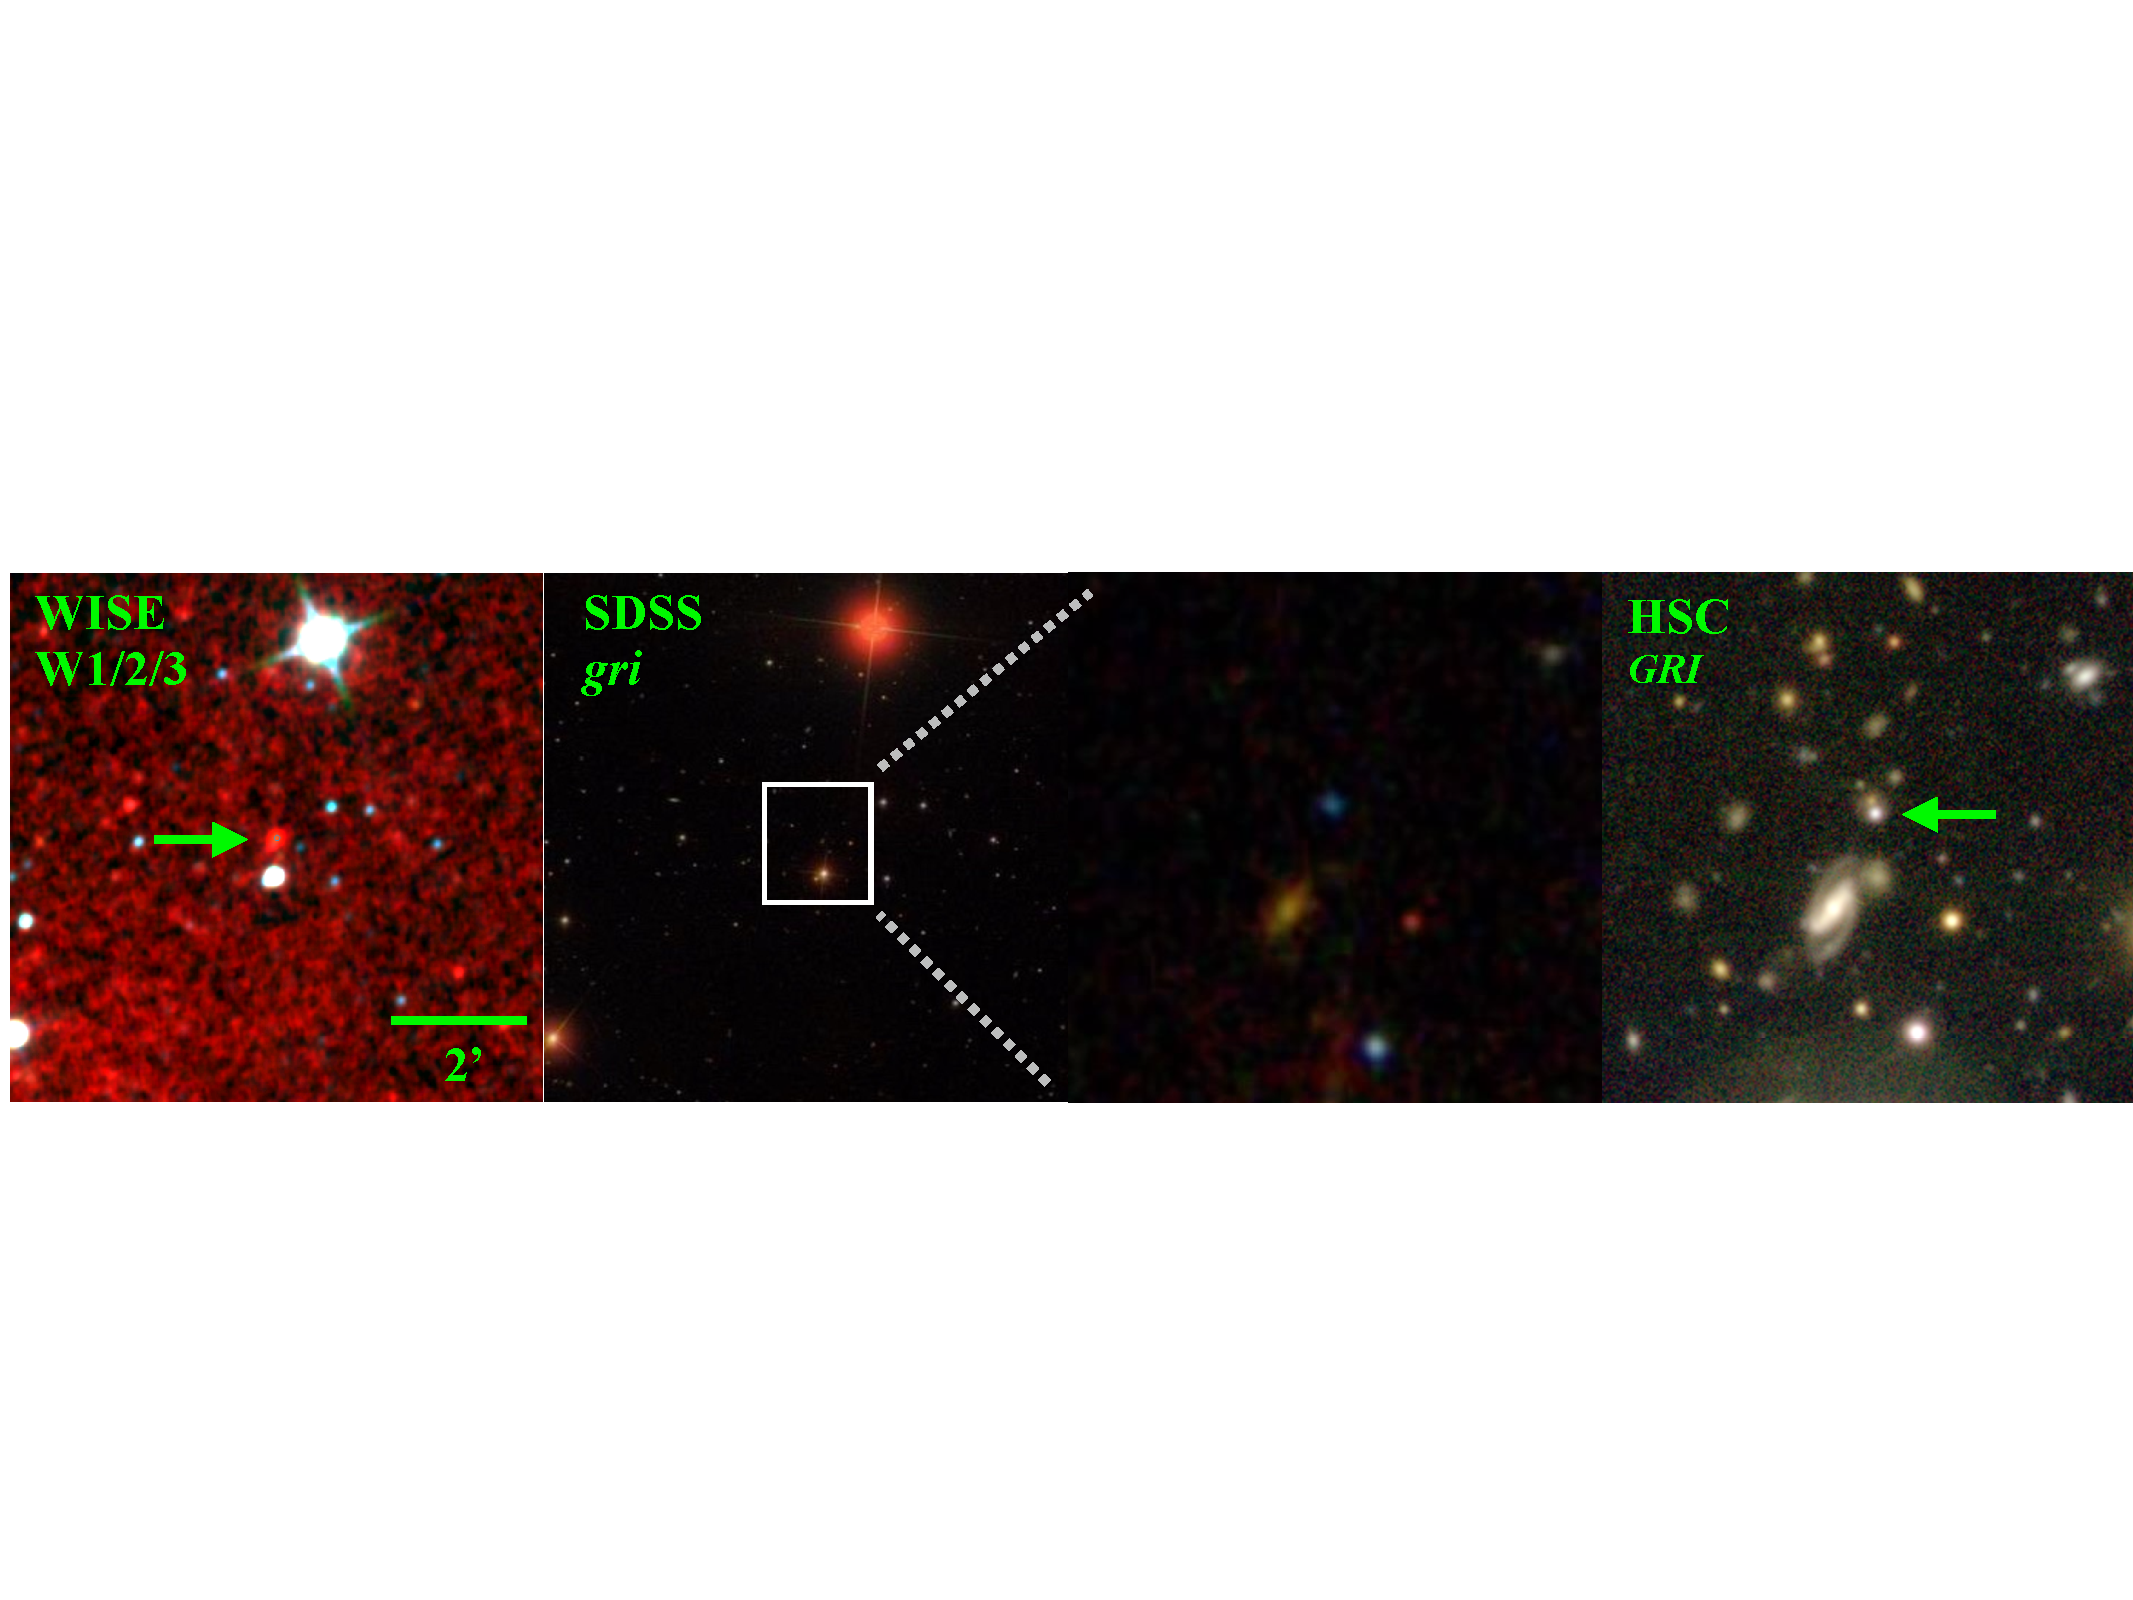
\includegraphics[width=17.0cm, trim={0.15cm 0 0.05cm 0},clip]
   {figures/WISE_SDSSzoomHSC_ERQ-image_v3.pdf}
    \vspace{-20pt}
   \caption{%\small   
\footnotesize 
%     \scriptsize
 %    \tiny
The IR and optical imaging of J2323-0100, an archetype of the
``Extremely Red Quasars'' (ERQs) at $z\approx2.5$ and a {\it JWST}
target. Shown are WISE {\it (left)}, where the quasar booms out as
indicated by the arrow; the SDSS image {\it (middle left)} with
zoom-in {\it (middle right)} on the optically faint source, and new
HSC imaging {\it (right)}, which shows tantalizing evidence for a
faint companion galaxy. Optical rest-frame spectra of J2323-0100,
revealed very broad (FWHM = 2500-5000 km s$^{-1}$), strongly
blue-shifted (by up to 1500 km s$^{-1}$) \oiii\ $\lambda$5007\AA\
emission lines in the ERQs. This is suggestive of active outflows and
potentially evidence for AGN feedback in action at the height of SMBH
activity.
}
  \vspace{-12pt}
 \label{fig:ERQ}
\end{center}
\end{figure}

\medskip
\medskip
\smallskip
\smallskip
\noindent
\textbf{\textsc{WP5: Observations of Quasars by the James Webb Space Telescope}} 

\smallskip
\smallskip
\noindent
In \citet{Ross2015} I discovered a new class of object, the ``extremely red
quasars'', that have optical spectroscopy from SDSS/BOSS, and
$r-[22\mu{\rm m}]>14$ colors (i.e., $F_{\nu,\, {\rm MIR}} / F_{\nu,\,
{\rm opt}} \gtrsim 1000$) from the Wide-field Infrared Survey Explorer
\citep[WISE;][]{Wright2010} satellite, see Figure~\ref{fig:ERQ}.  The ERQs are a
unique obscured quasar population with extreme physical conditions
related to powerful outflows across the line-forming regions. As my team 
have shown, these
sources are the signposts of the most dramatic form of quasar feedback
at the peak epoch of galaxy formation, and may represent an active
``blow-out'' phase of quasar evolution \citep{Zakamska2016, Hamann2017}.  
 However, due to
the current lack of access to mid-infrared spectroscopy, it is still
unknown whether the large IR luminosities observed in these quasars is
from star formation, which would produce strong polycyclic aromatic
hydrocarbon (PAH) spectral features, or, if it is from the hot dust
near the central quasar, which should produce much weaker/no PAH
emission.

\smallskip
\smallskip
\noindent
What are the star-formation properties of luminous quasars at the peak
of quasar activity?  We aim to answer this by looking for the presence
of polycyclic aromatic hydrocarbon (PAH) spectral features in infrared
bright quasars with the {\it James Webb Space Telescope} (JWST).  

\smallskip
\smallskip
\noindent
{\bf WP5 is high risk, high-reward.}  This is an ideal investigation for
the JWST, but we classify this as high-risk since we have to apply for
the telescope time and are not guaranteed the data.  We note this will
be the single WP NPR would lead and does not impact in any direct way
the other WPs. This would lead to very-high gain science.  

\smallskip
\smallskip
\noindent
{\bf Key
Deliverables:} State-of-the-art data products from the JWST, with the
observational evidence and physical interpretation of how ``quasar
feedback'' regulates galaxy formation in high-redshift quasars.
{\bf Timelime:} The deadline for JWST Cycle 1 GO programmes is 
06th April 2018, so I will know if I have been awarded observing 
time here before the start of the ERC. 


%%%
%%%   W P   6 
%%%
\medskip
\medskip
\smallskip
\smallskip
\noindent
\textbf{\textsc{WP6: New Object Discovery:}} 

\smallskip
\smallskip
\noindent
The LSST will scan the sky repeatedly, enabling it, and us, to both
discover new, distant transient events and to study variable objects
throughout our universe. The LSST will extend our view of the
changeable universe a thousand times over current surveys.  The most
interesting science to come may well be the discovery of new classes
of objects.

\smallskip
\smallskip
\noindent
By tapping into the massive raw discovery space that the new
experiments will open up, there is the highly likely outcome of
discovering something ``brand new'' \citep{Ivezic2008_LSST, 
LSST}. 
%%
This could include the electromagnetic counterparts to 
mergers of Binary SMBHs (with their associated gravitational wave
chirp and ringdown). After the discovery of GW1708017 \citep{GW170817} 
and its EM counterpart, \citep{GW170817_multi}, there has been 
considerable interest in using merging black holes as standard 
sirens, \citep[][]{GW170817_H0}. 
{\bf Q4D will have the ability to detect the EM signatures of 
the merging SMBHs. Whether they are detected in LIGO as well, 
will be exceptionally exciting to find out.}

\smallskip
\smallskip
\noindent
Objects potentially similar to repeating Fast Radio Bursts 
\citep{Spitler2016} or more objects akin to 
`SCP 06F6' \citep{Barbary2009} or 
`iPTF 16fnm' \citep{Miller2017} 
which are suggested to be supernova at the extremes of the
luminosity distribution, but are still not convincingly explained.


\smallskip
\smallskip
\noindent
{\bf WP6 is medium-risk, exceptionally high-reward.}  We class this as
medium-risk, since it is tricky to class a WP with essentially unknown
discovery potential as fully `low-risk'. However, we do not classify
this as `high-risk' since if there was a paucity of discovery of novel
classes of objects, this would be the first time in the history of
observational astrophysics that a new facility such as LSST has come
online and found nothing new.  

\smallskip
\smallskip
\noindent
{\bf Key Deliverables:} Potential
discovery of new classes of astronomical objects.
{\bf Timeline:} Peak Discovery Potential will come during the 
very early operation of LSST. We have to thus have {\tt QuasarSieve}, 
our ML light curve algorithms trained, and be ready 
to follow-up where necessary here. 


\medskip  \medskip \smallskip \smallskip \noindent
\subsection{Feasibility}

\smallskip
\smallskip
\noindent
By its inherent nature, our programme is high-risk and high-reward, but
we {\it fundamentally} have the personnel and skill sets that are 
necessary to make this project feasible. 
%% Mention your experience and knowledge to hedge against this risk or alternative approaches or help from collaborators. 
I have a track-record of managing scientific groups in 
large international and world-leading collaborations. {\it Critically, 
he also has a track record of developing key software packages 
on strict deadlines, e.g. the BOSS Quasar Target Selection software 
package (that contained a suite of novel ML algorithms).}
%
%% Have a dedicated section on feasibility of what you are proposing. Explain which WP’s/tasks present high levels of risk. 
%
%%Provide a contingency plan, particularly if any of the tasks are unconventional, present a great challenge and are high risk (but also high gain). 

%
%% Be ``safely adventurous''.  
%
%% Include a gantt chart or a timeline for the evaluators to visualise the timescale of each component of the work you are proposing.  Include a 4-5 line summary to recap and remind the evaluator what the essence of the project is and why it so important to get this funded now.







%%%%%%%%%%%%%%%%%%%%%%%%%%%%%%%%%%%%%%%%%%%%%%%%%%%%%%%%%%%%%%%%%%%%%%%%%%%%%%%
%%%%%%%%%%%%%%%%%%%%%%%%%%%%%%%%%%%%%%%%%%%%%%%%%%%%%%%%%%%%%%%%%%%%%%%%%%%%%%%
%%
%%
%%             c.     R  E  S  O  U  R  C  E  S 
%%
%%
%%%%%%%%%%%%%%%%%%%%%%%%%%%%%%%%%%%%%%%%%%%%%%%%%%%%%%%%%%%%%%%%%%%%%%%%%%%%%%%
%%%%%%%%%%%%%%%%%%%%%%%%%%%%%%%%%%%%%%%%%%%%%%%%%%%%%%%%%%%%%%%%%%%%%%%%%%%%%%%
\section{Resources (including project costs)}
Here we summarize and justify the budget.

\begin{figure}
  \begin{center}
    \hspace{-0.5cm}
    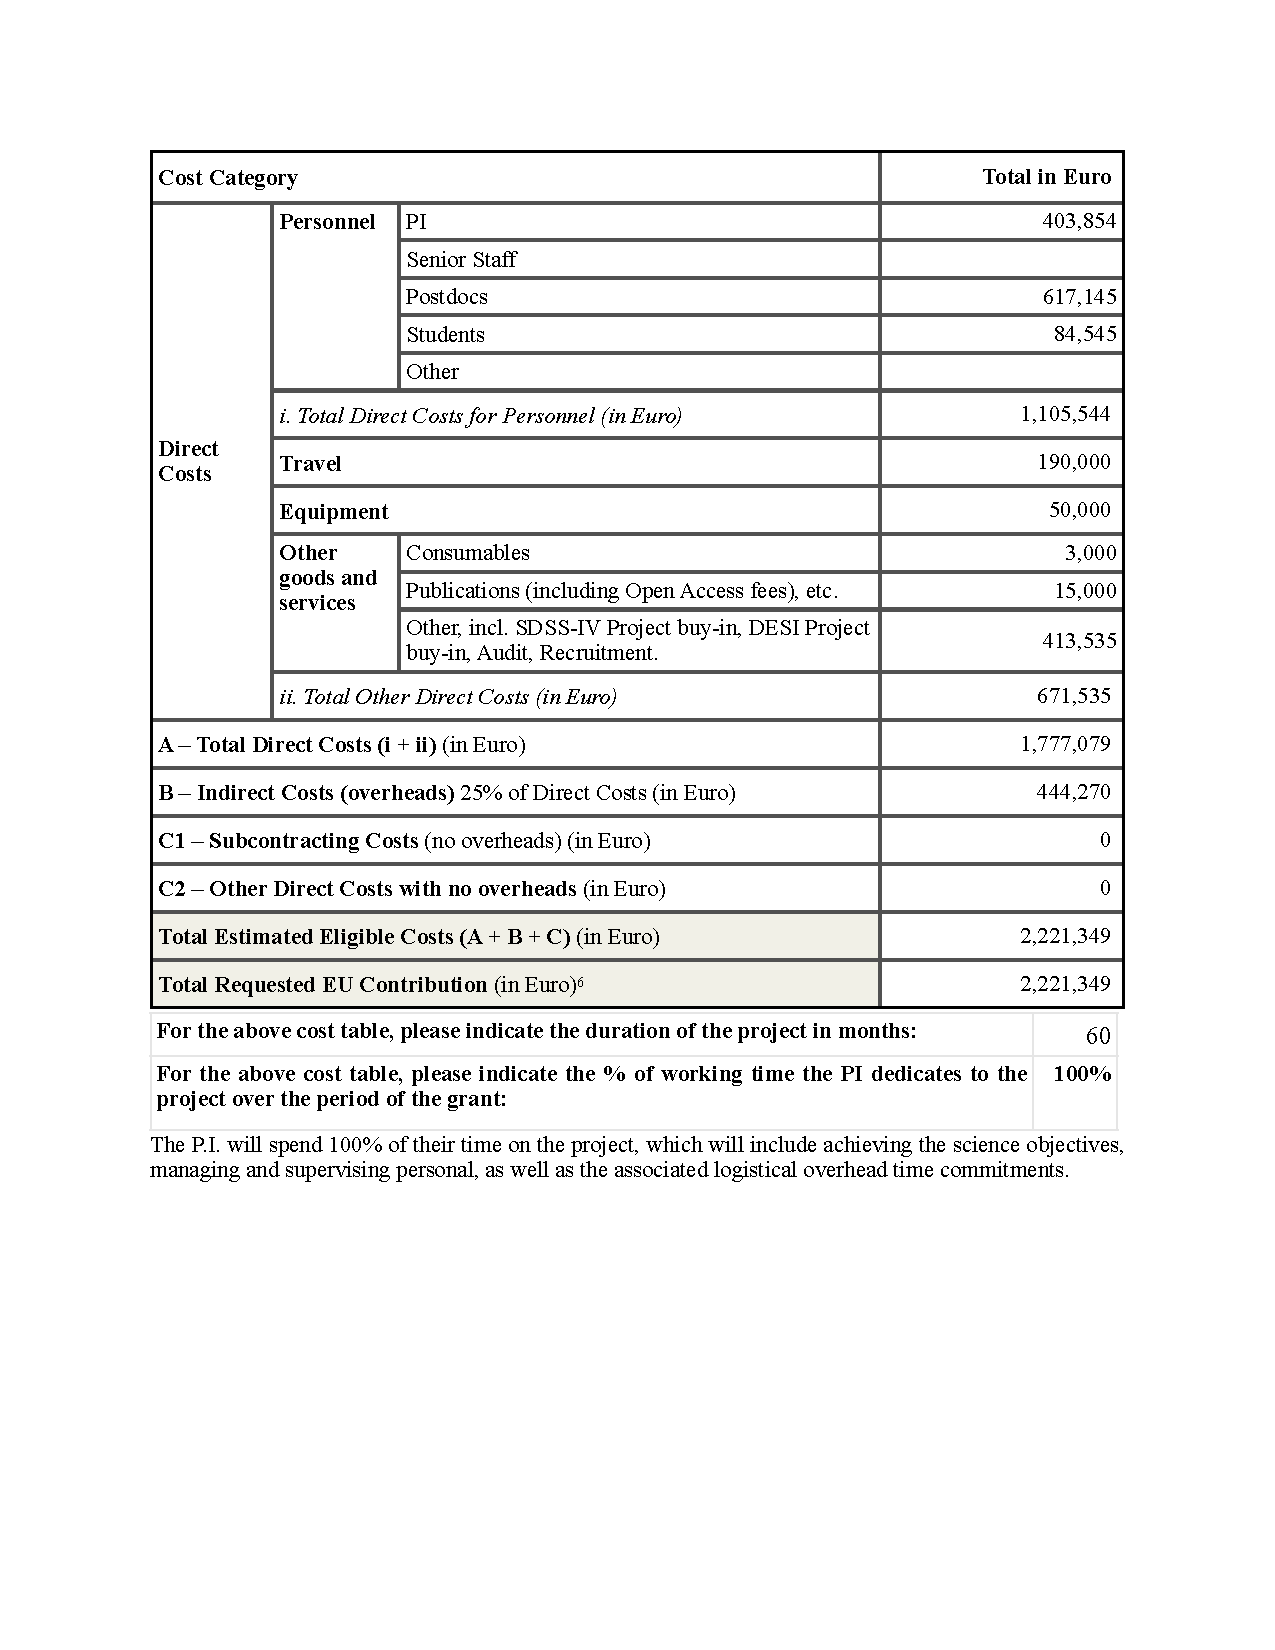
\includegraphics[width=16.6cm]
    {figures/ResourcesSummary.pdf}
    \vspace{-26pt}
 \label{fig:ResourcesSummary}
\end{center}
\end{figure}


\smallskip
\smallskip
\noindent
\textbf{\textsc{Team Composition:}}
Our team will consist of the PI, three postdoctoral research
associates (PDRAs), and 1 PhD student.  Two postdoctoral appointments
will be for three years each and one will be for a four year
appointment (a total of 10 FTE over 5 years).  The PhD student
will have a four year appointment.  The ambitious nature of this
project requires a large team of both observational and theoretical
postdoctoral scholars and PhD students to complete the proposed
research.  The PI is not a current member of academic staff and
therefore has no responsibilities extending beyond research.  As such,
the PI requests 100\% of his salary and, if successful, will focus solely on
the aims of the project.  Again, this will be necessary to achieve all
our goals on the given schedule.

\smallskip
\smallskip
\noindent
NPR is a world-leader in the field of extragalactic observational
astrophysics. NPR's research focuses on implementing novel data
science and machine learning algorithms and techniques in order to
discover and study the physical processes in quasars. I have an
exceptionally strong track record including being the lead of a
science Working Group, with prodigious scientific output
(\href{https://tinyurl.com/ycxd8lb6}{over 400 published, peer-reviewed
papers} from that particular collaboration).

\smallskip
\smallskip
\noindent
I was the Co-Founder and Chief Data Scientist of String Security
Inc. I built a predictive threat detection and remediation
platform for cyber security teams by applying machine learning and
predictive algorithms.  Thus the PI's research strengths, ability to
quickly develop bleeding-edge software and science output are all
ideally matched to this proposal.

\smallskip
\smallskip
\noindent
The skill set of PDRA1 would include development of the underlying
tools and techniques necessary to extract meaning from large and/or
complex data sets.  PDRA1 would have a strong physical sciences
background, and a PhD in astrophysics or computer science.  The skill
sets of PDRA2 would include expertise in time series analysis,
primarily with optical data but potentially also in other wavebands.
PDRA2 would have a PhD in astrophysics or a related field.  The skill
set of PDRA3 would include experience with fluid mechanics modelling
and/or large computer simulations.  PDRA3 would have a PhD in
astrophysics, mathematics or computer science.  PhD1 would have a
Masters or a strong 4-year undergraduate degree in Physics or
Mathematics with evidence of research-level project work.

\smallskip 
\smallskip
\noindent \textbf{\textsc{Salaries:}} The primary expenditure of our
project corresponds to salaries in order support the large team
necessary for this project.  The PI will be fully involved (project
management, scientific analysis, student supervision, postdoc
mentorship, proposal writing, communication with external
collaborations, and paper writing) and is covered at the 100\% level
over 5 years.  Salaries are determined according to the UEDIN salary
scale: \euro80.7k per FTE for the PI, \euro61.3k per FTE for the
PDRAs and \euro21.1k per FTE for PhD students.  The total cost of
salaries over 5 years is {\bf \euro 1106k}.

\smallskip 
\smallskip
\noindent \textbf{\textsc{Travel and Communication:}} 
A major expense is in the form of travel. I expect all group members
to disseminate our results in international conference but also to
participate in external collaboration meeting (at least one per year).
I am currently tax-payer funded, and a deep believer in letting
citizens know how their governments spend public money when investing
in scientific projects with potential impact on their lives and on
society.  Thus broad communication of this research project is a large
personal goal. Due to the nature and timing of our proposal, it will
almost certainly be critical for the PDRAs to have extended (several
week long) visits to the US and ESO Chile. I have allocated thus
allocated \euro10k/year for all members of the group for travel. This
level of commitment is necessary as has been proved by the PI's recent
and continued involvement with the e.g.  US-based surveys (and the
benefit to his research fellowship). The total travel budget is {\bf
\euro190k.}

\smallskip
\smallskip
\noindent
\textbf{\textsc{Publications:}}
Our work will be published in international journals such as Nature,
Nature Astronomy, Science, Monthly Notices of the Royal Astronomical
Society and the Astrophysical Journal. I have allocated \euro3k/year
for the cost of publications. In addition, all papers will be on the
arXiv preprint server free of charge. The total publications budget is
{\bf \euro15k.}

\smallskip
\smallskip
\noindent
\textbf{\textsc{Equipment \& Consumables:}} I have allocated
\euro10k/person for the initial purchase of a desktop and laptop
computer.  While we will have adequate resources to fully deploy {\tt
QuasarSieve} and will run our theory simulations on institute
(e.g. IfA Cullen), university
(e.g. \href{https://www.ed.ac.uk/information-services/research-support/research-computing/ecdf}{Edinburgh
Compute and Data Facility}) or national
{\href{https://www.hartree.stfc.ac.uk/Pages/home.aspx}{(The Hartree
Centre)} facilites, the rate limiting factor of our project and WPs
will be how quickly and efficiently we can deploy our new codes and
analysis.

\smallskip \smallskip
\noindent We require the budget for mid-to-high end hardware, (with
specifications that are not in the typical desktop the university
would supply) and also the e.g. large format displays that massively
boost productivity.  This can include having more than one
monitor 
(
%most programmers agree, and having experience this for myself, having 
e.g. 2 monitors leads to efficient coding, giving 
one full, often `portrait' monitor for code, and another for
documentation, specifications, StackOverflow help etc.)
Laptops are necessary for any extended time away (e.g. ``First Light' travel 
justified above) from the office. 
%\smallskip \smallskip \noindent 
Consumables are limited to \euro600/year (for the purchase
of back-up drives and other equipment). The total equipment and
consumables budget is {\bf \euro53k.}



\smallskip
\smallskip
\noindent
\textbf{\textsc{Access to Large Facilities:}}
We ask for additional funds that are available to cover ``access to
large facilities''.  We request support for the ``buy-in'' to two of
the new surveys, SDSS-V and DESI. The costs here are \euro184.1k and
\euro200.1k, respectively.
%%
We specifically request access to these
funds as it gives our project access to telescopes and data in the
North and Southern Hemispheres (for complete coverage of the celestial
sphere) and delivers the crucial early spectroscopy that will be vital
to train, test and build our data science and machine learning codes
and algorithms.  We emphasise that the science return is `exponential'
(rather than `linearly') dependent on the breadth of data available
and heralds a brand new regime of ``several-survey'' or
``multi-mission'' astronomy. 
Buy-in allows the two observational PDRAs along with the PhD student 
to have data access rights here and 
 {\it would place the
PI and the University of Edinburgh as the only group and institute
in the world to be involved in SDSS-V, DESI, 4MOST, LSST and ESA {\it
Euclid} and JWST}.
The total budget for the access to large facilities is {\bf \euro384.2k}.

\smallskip
\smallskip
\noindent
Total budget before facilities costs: \textbf{\underline{\euro 1,741,099}}. \\
Total budget including facilities costs: \textbf{\underline{\euro 2,221,349}}.\\




\newpage
%%\thispagestyle{empty}
\fancyhf{}
%\lhead{{\it ERC-2018-CoG}}
%\lhead{{\it DEQUASARS: Part B1 }}
\lhead{{\it Ross}}
\chead{Part B2}
\rhead{Q4D}
\setcounter{page}{1}
\lfoot{{\it ERC-COG-2018}}
\rfoot{{\it Scientific Proposal}}
%\cfoot{{\it Page \thepage\ of 5}}

%\newpage
\begin{center}
\medskip
 \medskip
 {\large \bf References}
    \vspace{-10pt}
\end{center}
\begin{multicols}{2}[]
\noindent
%\footnotesize
%\scriptsize
%\tiny
\lbrack 1\rbrack Kormendy \& Ho, 2013, ARAA, 51, 511\\
\lbrack 2\rbrack Kormendy,  2016, ASSL, 418, 431\\
\lbrack 3\rbrack Alexander et al., 2012, NewAR, 56, 93\\
\lbrack 4\rbrack King \& Pounds, 2015, ARAA, 53, 115 \\
\lbrack 5\rbrack Heckman \& Best, 2014, ARAA, 52, 589\\
\lbrack 6\rbrack Naab \& Ostriker, 2017, ARAA, 55, 59 \\
\lbrack 7\rbrack Netzer, 2015, ARAA, 53,  365\\
\lbrack 8\rbrack Padovani, 2017, A\&ARv, 25, 2\\
%%
\lbrack  9\rbrack Ata et al., 2017, arXiv1705.06373v2\\
\lbrack10\rbrack Solsar et al., 2013, JCAP, 04, 026 \\
\lbrack11\rbrack Busca et al.,  2013, A\&A, 552, 96 \\
\lbrack12\rbrack Delubac et al.,  2015, A\&A, 574, 59 \\
\lbrack13\rbrack Bautista et al., 2017, A\&A, 603, 12 \\
\lbrack14\rbrack du Mas des Bourboux et al., 2017, arXiv1708.02225v3\\
\lbrack15\rbrack Font-Riber et al., 2014, JCAP, 05, 027\\
%%
\lbrack16\rbrack Ross et al. 2015, MNRAS, 453, 3932\\
\lbrack17\rbrack Wright et al., 2010, AJ, 140, 1868\\
\lbrack18\rbrack Zakamska et al., 2016, MNRAS, 459, 3144\\
\lbrack19\rbrack Hamann et al., 2017, MNRAS, 464, 3431\\
%%
\lbrack20\rbrack Timlin, Ross et al., 2016, ApJS, 225, 1\\
\lbrack21\rbrack Timlin, Ross et al., 2017, ApJ, {\it in prep.}\\
%%
\lbrack22\rbrack LaMassa et al., 2015, ApJ, 800, 144\\
\lbrack23\rbrack Runnoe et al., 2016, MNRAS, 455, 1691\\
\lbrack24\rbrack Ruan et al, 2016, ApJ, 826, 188\\
\lbrack25\rbrack MacLeod, Ross et al., 2016, MNRAS, 457, 389\\
%%
\lbrack26\rbrack Meisner et al., 2017, AJ, 153, 38 \\
\lbrack27\rbrack Meisner et al., 2017, AJ, 154, 161 \\
% Meisner  et al., 2017, arXiv1710.02526v1 \\
\lbrack28\rbrack Ross et al., 2017, Nat.As., {\it in prep.} \\
%%
\lbrack29\rbrack Hopkins et al., 2006, ApJS, 163, 1\\
%%
\lbrack30\rbrack Schlegel et al., 2011,  arXiv:1106.1706v2 \\
%
\lbrack31\rbrack Ross et al., 2009, ApJ, 697, 1634 \\
%%
\lbrack32\rbrack Lombriser \& Taylor, 2016, JCAP, 03, 031 \\
\lbrack33\rbrack Baker et al, 2017,  arXiv1710.06394v1 \\
%%
\lbrack34\rbrack Watson et al.,  2011, ApJ, 740, L49\\
\lbrack35\rbrack King et al., 2014, MNRAS, 441, 3454\\
\lbrack36\rbrack King et al., 2015, MNRAS, 453, 1701\\
\lbrack37\rbrack Shen et al., 2015, ApJS, 216, 4\\
%\lbrack37\rbrack The Pierre Auger Collaboration, 2017, Science, 357, 6357 \\
\lbrack38\rbrack Hviding et al.,  2017, arXiv1711.01269v1 



\end{multicols}

\bibliographystyle{plainnat}
\bibliography{/cos_pc19a_npr/LaTeX/tester_mnras}




\end{document}

